\documentclass{beamer}

%\usetheme[frameno]{Arguelles}
%\usetheme{default}
\usetheme{Madrid}
\usetheme{default}
\usepackage{svg}
%\usepackage{minted}
\usepackage{adjustbox}
\usepackage{listings}
\usepackage{hyperref}

% \usepackage[utf8]{inputenc}
% \usepackage[russian]{babel}
\usepackage{graphicx}
\usepackage{blkarray}
% \usepackage{sidecap}
\usepackage{csquotes}
\usepackage{amsmath}
\usepackage{emoji}
\usepackage[backend=biber,hyperref=true,style=numeric]{biblatex}

% Установка цветов ссылок
\hypersetup{
    colorlinks=true,      % Включает цветные ссылки
    linkcolor=blue,      % Цвет ссылок на внутренние ссылки
    citecolor=blue,      % Цвет ссылок на цитаты
    urlcolor=blue        % Цвет ссылок на URL
}

% Настройки для Python кода
% Define style for Bash code
\lstdefinestyle{bashStyle}{
  language=Bash,
  basicstyle=\ttfamily\footnotesize,
  keywordstyle=\color{blue},
  commentstyle=\color{gray},
  stringstyle=\color{orange},
  showstringspaces=false,
  columns=flexible,
  numbers=left,
  numberstyle=\tiny\color{gray},
  backgroundcolor=\color{lightgray!20},
  frame=single,
  breaklines=true,
  captionpos=b,
  xleftmargin=1em,
  xrightmargin=1em
}

\hypersetup{
    colorlinks=true,
    linkcolor=blue,
    urlcolor=blue
}

% Define style for Python code
\lstdefinestyle{pythonStyle}{
  language=Python,
  basicstyle=\ttfamily\footnotesize,
  keywordstyle=\color{blue},
  commentstyle=\color{gray},
  stringstyle=\color{orange},
  showstringspaces=false,
  columns=flexible,
  numbers=left,
  numberstyle=\tiny\color{gray},
  backgroundcolor=\color{lightgray!20},
  frame=single,
  breaklines=true,
  captionpos=b,
  xleftmargin=1em,
  xrightmargin=1em
}

% Добавление поддержки русского языка
\usepackage[utf8]{inputenc} % UTF-8 кодировка
\usepackage[russian, english]{babel} % Поддержка русского и английского языков
\usepackage{tikz}

\title{NLP basics}
%\subtitle{Overview}
\author{Vasily Konovalov, Andrei Glinskii}
\date{}
\addbibresource{./references.bib}


\begin{document}

\frame[plain]{\titlepage}

\begin{frame}{Table of Contents}
    \tableofcontents
\end{frame}

\section{Regex}

\begin{frame}
    \frametitle{Regular Expressions introduction}
    \begin{itemize}
        \item A regular expression (regex) is a sequence of characters defining a search pattern.
        \item Commonly used for pattern matching in strings.
        \item Useful in data validation, text parsing, and complex search operations.
    \end{itemize}
\end{frame}

\begin{frame}
    \frametitle{Python's `re` Module}
    \begin{itemize}
        \item Python provides the `re` module to work with regular expressions.
        \item Main functions:
        \begin{itemize}
            \item \texttt{re.match()} - Checks for a match only at the beginning of the string.
            \item \texttt{re.search()} - Searches the entire string for a match.
            \item \texttt{re.findall()} - Returns all matches in a list.
            \item \texttt{re.finditer()} - Returns an iterator yielding match objects.
            \item \texttt{re.sub()} - Replaces matches with a specified string.
        \end{itemize}
    \end{itemize}
\end{frame}

\begin{frame}
    \frametitle{Basic Syntax}
    \begin{itemize}
        \item \textbf{Literal Characters:} `a`, `b`, `1`, `*`
        \item \textbf{Metacharacters:}
        \begin{itemize}
            \item \texttt{.} - Matches any character except newline.
            \item \texttt{^} - Matches the start of the string.
            \item \texttt{\$} - Matches the end of the string.
            \item \texttt{[]}- Matches any one of the enclosed characters.
            \item \texttt{()} - Groups expressions.
            \item \texttt{|} - OR operator.
        \end{itemize}
    \end{itemize}
\end{frame}

\begin{frame}
    \frametitle{Quantifiers}
    \begin{itemize}
        \item \textbf{*} - Matches 0 or more occurrences.
        \item \textbf{+} - Matches 1 or more occurrences.
        \item \textbf{?} - Matches 0 or 1 occurrence.
        \item \textbf{\{n\}} - Matches exactly n occurrences.
        \item \textbf{\{n,m\}} - Matches between n and m occurrences.
    \end{itemize}
\end{frame}

\begin{frame}[fragile]
    \frametitle{Examples}
    \begin{lstlisting}[style=pythonStyle, caption=Using Regular Expressions]
import re

pattern = r'\b(\d{2}/\d{2}/\d{4})\b'
text = 'The event is on 12/25/2024.'
matches = re.findall(pattern, text)
print(matches)
    \end{lstlisting}
\end{frame}

\begin{frame}[fragile]
    \frametitle{Examples}
    \begin{lstlisting}[style=pythonStyle, caption=Matching Email Addresses]
import re

pattern = r'\b[A-Za-z0-9._%+-]+@[A-Za-z0-9.-]+\.[A-Z|a-z]{2,}\b'
text = 'Contact us at example@example.com'
matches = re.findall(pattern, text)
print(matches)
    \end{lstlisting}
\end{frame}

\begin{frame}
    \frametitle{Common Pitfalls}
    \begin{itemize}
        \item Forgetting to escape special characters.
        \item Misunderstanding the difference between greedy and non-greedy matching.
        \item Overly complex regular expressions that are difficult to read and maintain.
    \end{itemize}
\end{frame}

\begin{frame}
    \frametitle{Regular Expressions conclusion}
    \begin{itemize}
        \item Regular expressions are a powerful tool for string manipulation.
        \item Python’s `re` module provides various functions to work with regex patterns.
        \item Practice with different patterns and functions to master regex.
        \item \href{https://habr.com/ru/articles/349860/}{Habr regex}
    \end{itemize}
\end{frame}


\section{Text normalization}

\begin{frame}
    \frametitle{Text normalization introduction}
    \begin{itemize}
        \item Text normalization is the process of transforming text into a standard form.
        \item Essential for improving consistency and reducing noise in text data.
        \item Commonly used in preprocessing steps in Natural Language Processing (NLP) tasks.
    \end{itemize}
\end{frame}

\begin{frame}
    \frametitle{Why Text Normalization is Important}
    \begin{itemize}
        \item Reduces variations in text, making it easier to analyze and model.
        \item Helps in handling issues like spelling errors, punctuation, and case sensitivity.
        \item Improves the quality of NLP models by providing clean, consistent input.
    \end{itemize}
\end{frame}

\begin{frame}
    \frametitle{Common Text Normalization Methods}
    \begin{itemize}
        \item \textbf{Lowercasing}: Converts all characters to lowercase.
        \item \textbf{Removing Punctuation}: Eliminates punctuation marks.
        \item \textbf{Stemming}: Reduces words to their root forms (e.g., "running" → "run").
        \item \textbf{Lemmatization}: Converts words to their base forms based on their meaning (e.g., "better" → "good").
        \item \textbf{Removing Stopwords}: Removes common words that provide little semantic value (e.g., "the", "and").
    \end{itemize}
\end{frame}

\begin{frame}[fragile]
    \frametitle{Lowercasing Example}
    \begin{itemize}
        \item Converts all characters in a text to lowercase.
        \item Useful for standardizing text, especially in case-insensitive tasks.
    \end{itemize}
    \begin{lstlisting}[style=pythonStyle, caption=Lowercasing in Python]

    text = "The Quick Brown Fox Jumps Over The Lazy Dog."

    # Convert text to lowercase
    normalized_text = text.lower()

    print(normalized_text)
    \end{lstlisting}
\end{frame}

\begin{frame}[fragile]
    \frametitle{Removing Punctuation Example}
    \begin{itemize}
        \item Removes punctuation marks such as periods, commas, and exclamation points.
        \item Helps in cleaning up text for further analysis.
    \end{itemize}
    \begin{lstlisting}[style=pythonStyle, caption=Removing Punctuation in Python]

    import string

    text = "Hello, world! How's everything?"

    # Remove punctuation
    normalized_text = text.translate(str.maketrans("", "", string.punctuation))

    print(normalized_text)
    \end{lstlisting}
\end{frame}

\begin{frame}[fragile]
    \frametitle{Stemming Example}
    \begin{itemize}
        \item Reduces words to their root forms.
        \item Useful in reducing inflectional forms and derivationally related forms of a word.
    \end{itemize}
    \begin{lstlisting}[style=pythonStyle, caption=Stemming in Python with NLTK]

    from nltk.stem import PorterStemmer

    stemmer = PorterStemmer()
    words = ["running", "jumps", "easily", "fairly"]

    # Perform stemming
    stems = [stemmer.stem(word) for word in words]

    print(stems)
    \end{lstlisting}
\end{frame}

\begin{frame}[fragile]
    \frametitle{Lemmatization Example}
    \begin{itemize}
        \item Converts words to their base or dictionary forms (lemmas).
        \item Takes into account the meaning of the word, unlike stemming.
    \end{itemize}
    \begin{lstlisting}[style=pythonStyle, caption=Lemmatization in Python with NLTK]

    from nltk.stem import WordNetLemmatizer
    from nltk.corpus import wordnet

    lemmatizer = WordNetLemmatizer()
    words = ["better", "running", "jumps"]

    # Perform lemmatization
    lemmas = [lemmatizer.lemmatize(word, pos=wordnet.VERB) for word in words]

    print(lemmas)
    \end{lstlisting}
\end{frame}

\begin{frame}[fragile]
    \frametitle{Removing Stopwords Example}
    \begin{itemize}
        \item Removes common words that provide little semantic meaning (e.g., "the", "is").
        \item Helps in focusing on the more meaningful words in the text.
    \end{itemize}
    \begin{lstlisting}[style=pythonStyle, caption=Removing Stopwords in Python with NLTK]
    from nltk.corpus import stopwords
    from nltk.tokenize import word_tokenize

    text = "This is a simple example showing how to remove stopwords."

    words = word_tokenize(text)

    stop_words = set(stopwords.words("english"))
    filtered_words = [word for word in words if word.lower() not in stop_words]

    print(filtered_words)
    \end{lstlisting}
\end{frame}

\begin{frame}
    \frametitle{Text normalization conclusion}
    \begin{itemize}
        \item Text normalization is a crucial preprocessing step in NLP.
        \item The methods discussed improve the quality of the input text for downstream tasks.
        \item Choosing the right combination of normalization techniques can significantly impact model performance.
    \end{itemize}
\end{frame}

\section{Tokenization}

\begin{frame}
    \frametitle{Tokenization introduction}
    \begin{itemize}
        \item Tokenization is the process of splitting text into individual units, called tokens.
        \item Tokens can be words, phrases, or even characters, depending on the level of granularity.
        \item Essential for many NLP tasks such as text classification, sentiment analysis, and machine translation.
    \end{itemize}
\end{frame}

\begin{frame}
    \frametitle{Why Tokenization is Important}
    \begin{itemize}
        \item Converts raw text into a format suitable for analysis.
        \item Helps in standardizing text data by breaking it into manageable pieces.
        \item Facilitates feature extraction and the application of various NLP models.
    \end{itemize}
\end{frame}

\begin{frame}
    \frametitle{Types of Tokenization}
    \begin{itemize}
        \item \textbf{Word Tokenization}
        \begin{itemize}
            \item Splits text into individual words.
            \item Example: "The quick brown fox" → ["The", "quick", "brown", "fox"]
        \end{itemize}
        \item \textbf{Subword Tokenization}
        \begin{itemize}
            \item Splits text into subword units or morphemes.
            \item Useful for handling out-of-vocabulary words.
            \item \textbf{Example:}
            \begin{itemize}
                \item Text: "tokenization"
                \item Subwords: ["token", "ization"]
                \item Method: Byte-Pair Encoding (BPE)
            \end{itemize}
        \end{itemize}
        \item \textbf{Character Tokenization}
        \begin{itemize}
            \item Splits text into individual characters.
            \item Example: "fox" → ["f", "o", "x"]
        \end{itemize}
    \end{itemize}
\end{frame}


\begin{frame}[fragile]
    \frametitle{Word Tokenization}
    \begin{itemize}
        \item Simple and straightforward.
        \item Commonly used with whitespace and punctuation as delimiters.
        \item Tools: \texttt{nltk.word\_tokenize()}, \texttt{spaCy}, \texttt{scikit-learn}
    \end{itemize}
    \begin{lstlisting}[style=pythonStyle, caption=nltk.tokenize]

    import nltk

    nltk.download('punkt')

    from nltk.tokenize import word_tokenize

    text = "The quick brown fox jumps over the lazy dog."

    tokens = word\_tokenize(text)

    print(tokens)
    \end{lstlisting}
\end{frame}

\begin{frame}[fragile]
    \frametitle{Subword Tokenization}
    \begin{itemize}
        \item Breaks words into subword units.
        \item Helps with handling rare and out-of-vocabulary words.
        \item Tools: Byte-Pair Encoding (BPE), SentencePiece, WordPiece.
    \end{itemize}
    \begin{lstlisting}[style=pythonStyle, caption=transformers 01]
        from transformers import AutoTokenizer

        # Load a pre-trained tokenizer, e.g., BERT

        tokenizer = AutoTokenizer.from_pretrained("bert-base-uncased")

        # Sample text
        text = "Tokenization in NLP is crucial for handling text data."

    \end{lstlisting}
\end{frame}

\begin{frame}[fragile]
    \frametitle{Subword Tokenization}
    \begin{lstlisting}[style=pythonStyle, caption=transformers 02]
        # Tokenize the text
        tokens = tokenizer.tokenize(text)

        print("Tokens:", tokens)

        # Convert tokens to input IDs (integer representation)
        input_ids = tokenizer.convert_tokens_to_ids(tokens)
        print("Input IDs:", input_ids)

        # Convert input IDs back to tokens (for verification)

        decoded_tokens = tokenizer.convert_ids_to_tokens(input_ids)

        print("Decoded Tokens:", decoded_tokens)
    \end{lstlisting}
\end{frame}


\begin{frame}[fragile]
    \frametitle{Character Tokenization}
    \begin{itemize}
        \item Breaks text into individual characters.
        \item Useful for languages with no clear word boundaries or when focusing on fine-grained analysis.
        \item Tools: Simple Python implementation, custom tokenization methods.
    \end{itemize}
    \begin{lstlisting}[style=pythonStyle, caption=Character Tokenization]

    # Sample text
    text = "The quick brown fox jumps over the lazy dog."

    # Character tokenization: Split text into characters
    tokens = list(text)

    print(tokens)
    \end{lstlisting}
\end{frame}

\begin{frame}
\frametitle{Subword Tokenization in detail}
Subword tokenization is a technique used in natural language processing to split text into smaller, more manageable units. This approach helps in handling out-of-vocabulary words and improving the performance of machine learning models. Common subword tokenization algorithms include:
\begin{itemize}
    \item Byte-Pair Encoding (BPE)
    \item Unigram Language Model
    \item SentencePiece
    \item WordPiece
\end{itemize}
\end{frame}

\begin{frame}
\frametitle{Byte-Pair Encoding (BPE)}
\begin{itemize}
    \item A data compression technique adapted for subword tokenization.
    \item Iteratively replaces the most frequent pair of characters with a new symbol.
    \item Example:
    \begin{itemize}
        \item Input: "low low lower lowest"
        \item Tokens: "low", "low", "low", "e", "r", "low", "e", "s", "t"
    \end{itemize}
\end{itemize}
\end{frame}

\begin{frame}
\frametitle{Unigram Language Model}
\begin{itemize}
    \item A probabilistic approach to subword tokenization.
    \item Trains a language model to determine the most probable subword units.
    \item Example:
    \begin{itemize}
        \item Input: "reading"
        \item Tokens: "re", "ad", "ing"
    \end{itemize}
\end{itemize}
\end{frame}

\begin{frame}
\frametitle{SentencePiece}
\begin{itemize}
    \item A versatile subword tokenizer developed by Google.
    \item Uses a variant of BPE or unigram model.
    \item Trains on raw text and produces a vocabulary of subwords.
    \item Example:
    \begin{itemize}
        \item Input: "Tokenization"
        \item Tokens: "Tok", "en", "ization"
    \end{itemize}
\end{itemize}
\end{frame}

\begin{frame}
\frametitle{WordPiece}
\begin{itemize}
    \item Developed by Google for the BERT model.
    \item Similar to BPE but uses a different training objective.
    \item Example:
    \begin{itemize}
        \item Input: "unhappiness"
        \item Tokens: "un", "happiness"
    \end{itemize}
\end{itemize}
\end{frame}

\begin{frame}
\frametitle{Comparison of Algorithms}
\scriptsize
\begin{tabular}{|l|p{3.5cm}|p{3.5cm}|}
\hline
Algorithm & Strengths & Weaknesses \\
\hline
BPE & Simple, effective for many languages & Can produce longer tokens for infrequent words \\
\hline
Unigram & Probabilistic, captures subword frequency & May not handle rare words as well \\
\hline
SentencePiece & Versatile, works well with various languages & Complexity of implementation \\
\hline
WordPiece & Effective for large-scale models & Requires a large training corpus \\
\hline
\end{tabular}
\end{frame}

\begin{frame}
    \frametitle{Tokenization Challenges}
    \begin{itemize}
        \item Handling punctuation and special characters.
        \item Managing different languages and their unique tokenization needs.
        \item Dealing with abbreviations, contractions, and named entities.
    \end{itemize}
\end{frame}

\begin{frame}
    \frametitle{Tokenization conclusion}
    \begin{itemize}
        \item Tokenization is a crucial step in NLP pipelines.
        \item The choice of tokenization method depends on the specific NLP task and data characteristics.
        \item Understanding and applying the right tokenization technique can significantly impact model performance.
        \item More at \href{https://huggingface.co/docs/transformers/tokenizer_summary}{HF tokenizer summary}
    \end{itemize}
\end{frame}

\section{BoW}

\begin{frame}
    \frametitle{Bag of Words introduction}
    \begin{itemize}
        \item Bag of Words (BoW) is a fundamental technique for representing text in NLP.
        \item It represents text as an unordered collection of words, disregarding grammar and word order.
        \item Commonly used for text classification and retrieval tasks.
    \end{itemize}
\end{frame}

\begin{frame}
    \frametitle{How Bag of Words (BoW) Works}
    \begin{itemize}
        \item Create a vocabulary from all unique words in the corpus.
        \item Represent each document as a vector of word frequencies from the vocabulary.
        \item Each element in the vector represents the count of a word in the document.
    \end{itemize}
\end{frame}

\begin{frame}
    \frametitle{Example of Bag of Words}
    \begin{itemize}
        \item Consider two sentences:
        \begin{itemize}
            \item Sentence 1: "The cat sat on the mat."
            \item Sentence 2: "The dog sat on the log."
        \end{itemize}
        \item Vocabulary: [the, cat, sat, on, mat, dog, log]
        \item Vector for Sentence 1: [2, 1, 1, 1, 1, 0, 0]
        \item Vector for Sentence 2: [2, 0, 1, 1, 0, 1, 1]
    \end{itemize}
\end{frame}

\begin{frame}
    \begin{figure}
        \centering
        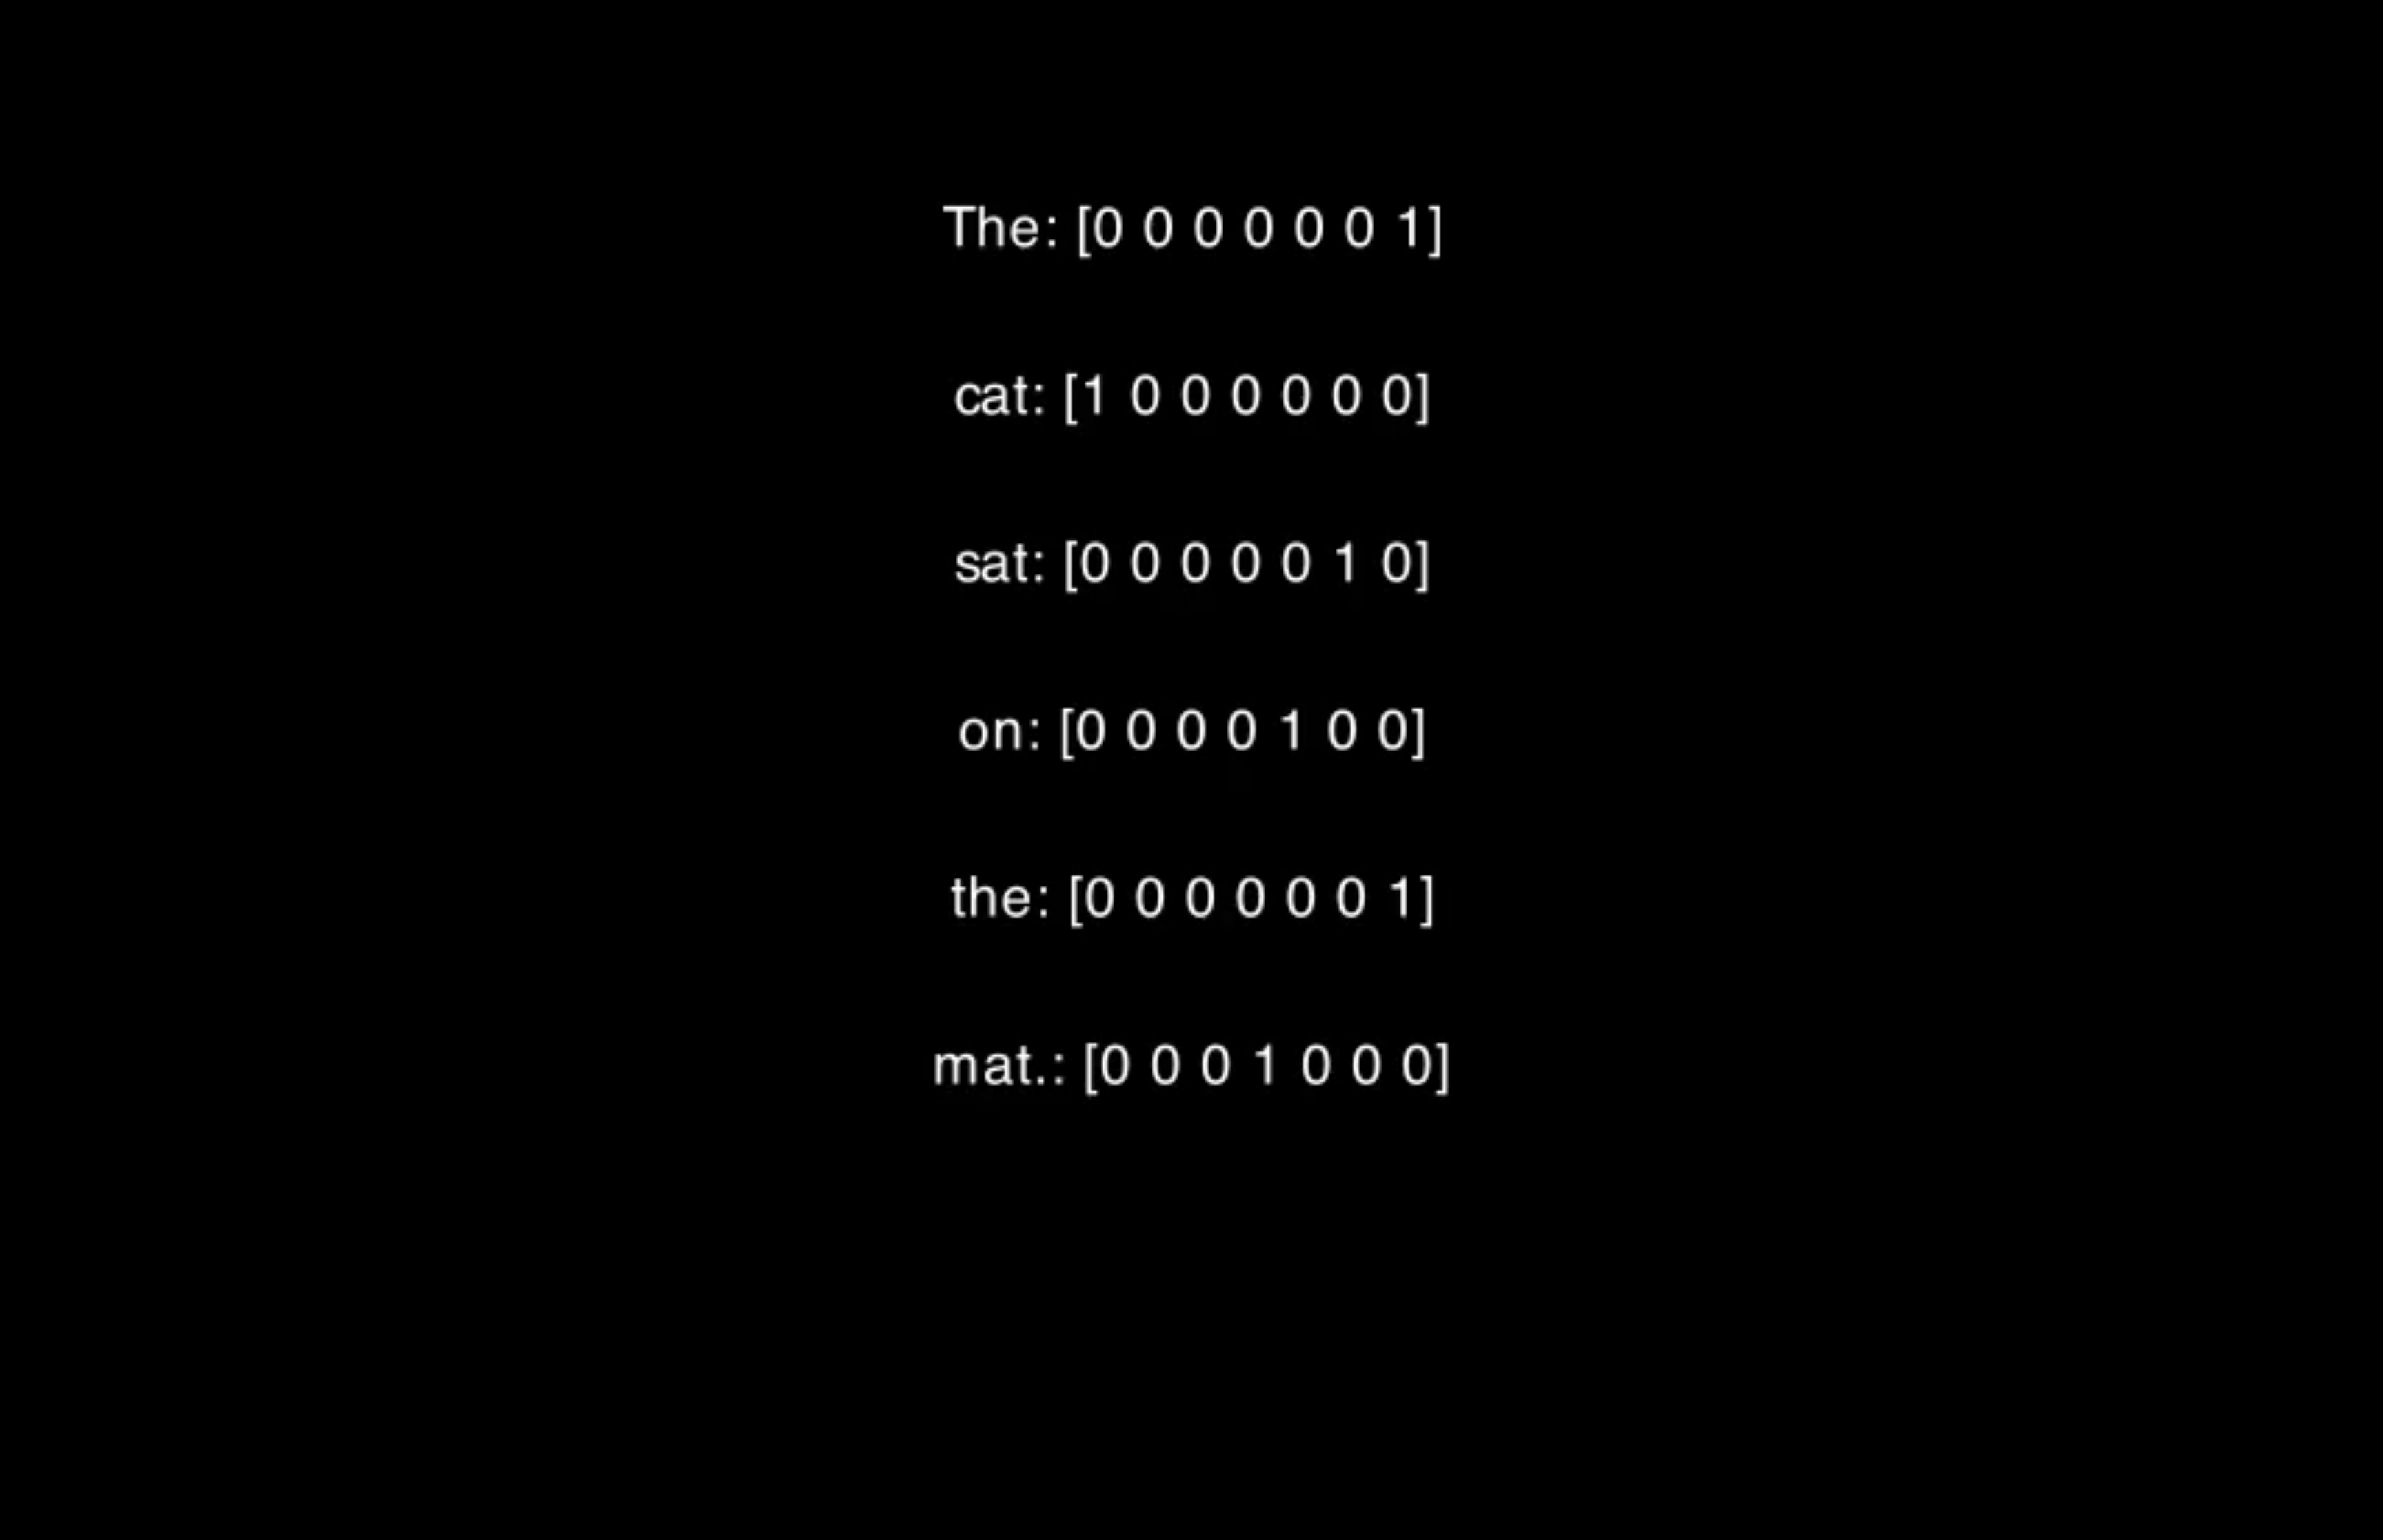
\includegraphics[width=1\textwidth,keepaspectratio]{images/ohe}
%        \caption{}
        \label{fig:ohe}
    \end{figure}
\end{frame}

\begin{frame}
    \frametitle{Advantages of Bag of Words (BoW)}
    \begin{itemize}
        \item Simple and easy to implement.
        \item Effective for text classification tasks.
        \item Works well with traditional machine learning algorithms.
    \end{itemize}
\end{frame}

\begin{frame}
    \frametitle{Limitations of Bag of Words (BoW)}
    \begin{itemize}
        \item Ignores word order and context.
        \item High-dimensional representations for large vocabularies.
        \item Cannot capture semantic meaning or relationships between words.
        \item No natural notion of similarity for BoW.
    \end{itemize}
\end{frame}

\begin{frame}[fragile]
    \frametitle{Bag of Words Example in Python}
    \begin{lstlisting}[style=pythonStyle, caption=Bag of Words with CountVectorizer 01]
        import re
        from sklearn.feature_extraction.text import CountVectorizer

        # Sample documents
        documents = [
        "The cat sat on the mat.",
        "The dog sat on the log!"
        ]

        # Custom preprocessing function
        def custom_preprocessor(text):
            # lowercasing
            text = text.lower()
            # Punctuation deletion
            text = re.sub(r'[^\w\s]', '', text)
            return text
    \end{lstlisting}
\end{frame}

\begin{frame}[fragile]
    \frametitle{Bag of Words Example in Python}
    \begin{lstlisting}[style=pythonStyle, caption=Bag of Words with CountVectorizer 02]
        # Create the Bag of Words model with the custom preprocessor
        vectorizer = CountVectorizer(preprocessor=custom_preprocessor)
        bow_matrix = vectorizer.fit_transform(documents)

        # Convert to array for easy viewing
        print(bow_matrix.toarray())

        # Display the vocabulary
        print(vectorizer.get_feature_names_out())
    \end{lstlisting}
\end{frame}

\begin{frame}[fragile]
    \frametitle{Bag of Words Example in Python}
    \begin{lstlisting}[style=pythonStyle, caption=Bag of Words with CountVectorizer 03]
        # Get feature names (words)
        feature_names = vectorizer.get_feature_names_out()

        # Create a key-value map (word to index)
        word_to_index = {word: idx for idx, word in enumerate(feature_names)}

        # Print the key-value map
        print("Word to Index Map:")
        for word, idx in word_to_index.items():
            print(f"{word}: {idx}")
    \end{lstlisting}
\end{frame}

\begin{frame}
    \frametitle{Understanding the Output}
    \begin{itemize}
        \item The output of `CountVectorizer` is a sparse matrix where each row represents a document and each column represents a word from the vocabulary.
        \item Each value in the matrix represents the frequency of a word in the corresponding document.
    \end{itemize}
\end{frame}

\begin{frame}
    \frametitle{Bag of Words conclusion}
    \begin{itemize}
        \item Bag of Words (BoW) is a simple and effective text representation technique.
        \item Despite its limitations, it is widely used in traditional machine learning tasks for text classification.
        \item More advanced techniques, such as TF-IDF and word embeddings, build upon the foundations of BoW.
    \end{itemize}
\end{frame}


\section{Naive Bayes}

\begin{frame}
    \frametitle{Naive Bayes introduction}
    \begin{itemize}
        \item Naive Bayes is a probabilistic classifier based on Bayes' Theorem.
        \item It assumes that the features are conditionally independent given the class.
        \item Widely used in text classification tasks such as spam detection and sentiment analysis.
    \end{itemize}
\end{frame}

\begin{frame}
    \frametitle{Naive Bayes Classifier}
    \begin{block}{Bayes' Theorem}
        \[
        P(C | X) = \frac{P(X | C) \cdot P(C)}{P(X)}
        \]
        where:
        \begin{itemize}
            \item \( P(C | X) \) is the posterior probability of class \( C \) given features \( X \).
            \item \( P(X | C) \) is the likelihood of features \( X \) given class \( C \).
            \item \( P(C) \) is the prior probability of class \( C \).
            \item \( P(X) \) is the marginal probability of features \( X \).
        \end{itemize}
    \end{block}
\end{frame}

\begin{frame}
    \frametitle{Naive Assumption}
    \begin{block}{Conditional Independence}
        The Naive Bayes classifier assumes that the features are conditionally independent given the class:
        \[
        P(X | C) = \prod_{i=1}^{n} P(x_i | C)
        \]
        where \( x_i \) are the individual features.
    \end{block}
\end{frame}

\begin{frame}
    \frametitle{Types of Naive Bayes Classifiers}
    \begin{itemize}
        \item \textbf{Multinomial Naive Bayes}
        \begin{itemize}
            \item Suitable for discrete features (e.g., word counts).
            \item Often used in text classification.
        \end{itemize}
        \item \textbf{Bernoulli Naive Bayes}
        \begin{itemize}
            \item Suitable for binary/boolean features.
            \item Example: presence/absence of words.
        \end{itemize}
        \item \textbf{Gaussian Naive Bayes}
        \begin{itemize}
            \item Assumes features follow a normal distribution.
            \item Suitable for continuous features.
        \end{itemize}
    \end{itemize}
\end{frame}

\begin{frame}
    \frametitle{Example: Text Classification}
    \begin{itemize}
        \item We will use the Multinomial Naive Bayes classifier to classify text.
        \item Example: Spam vs. Not Spam classification.
    \end{itemize}
\end{frame}

\begin{frame}
    \frametitle{Example: Text Classification}
    \begin{figure}
        \centering
        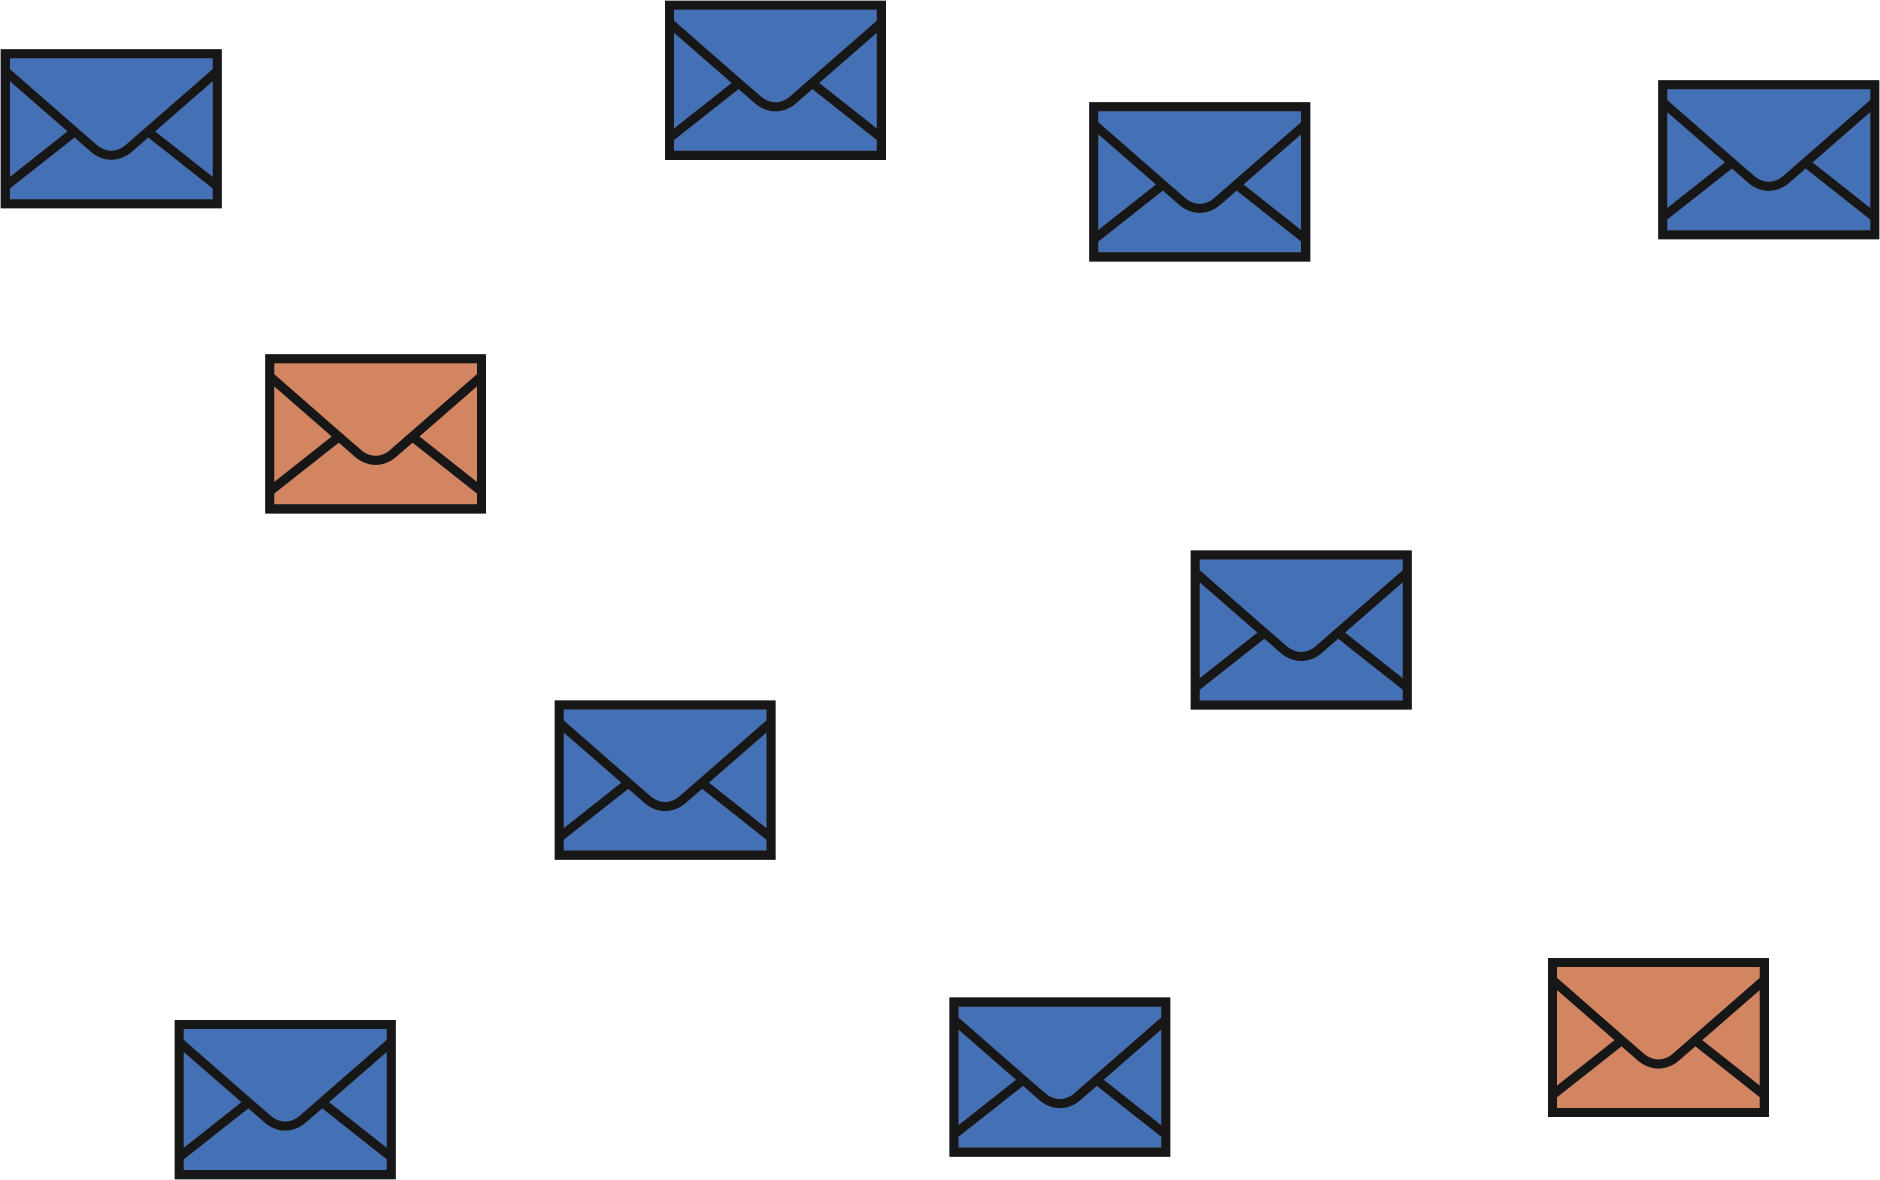
\includegraphics[width=1\textwidth,keepaspectratio]{images/spam01}
        \caption{}
        \label{fig:spam01}
    \end{figure}

\end{frame}

\begin{frame}
    \frametitle{Example: Text Classification}
    \begin{figure}
        \centering
        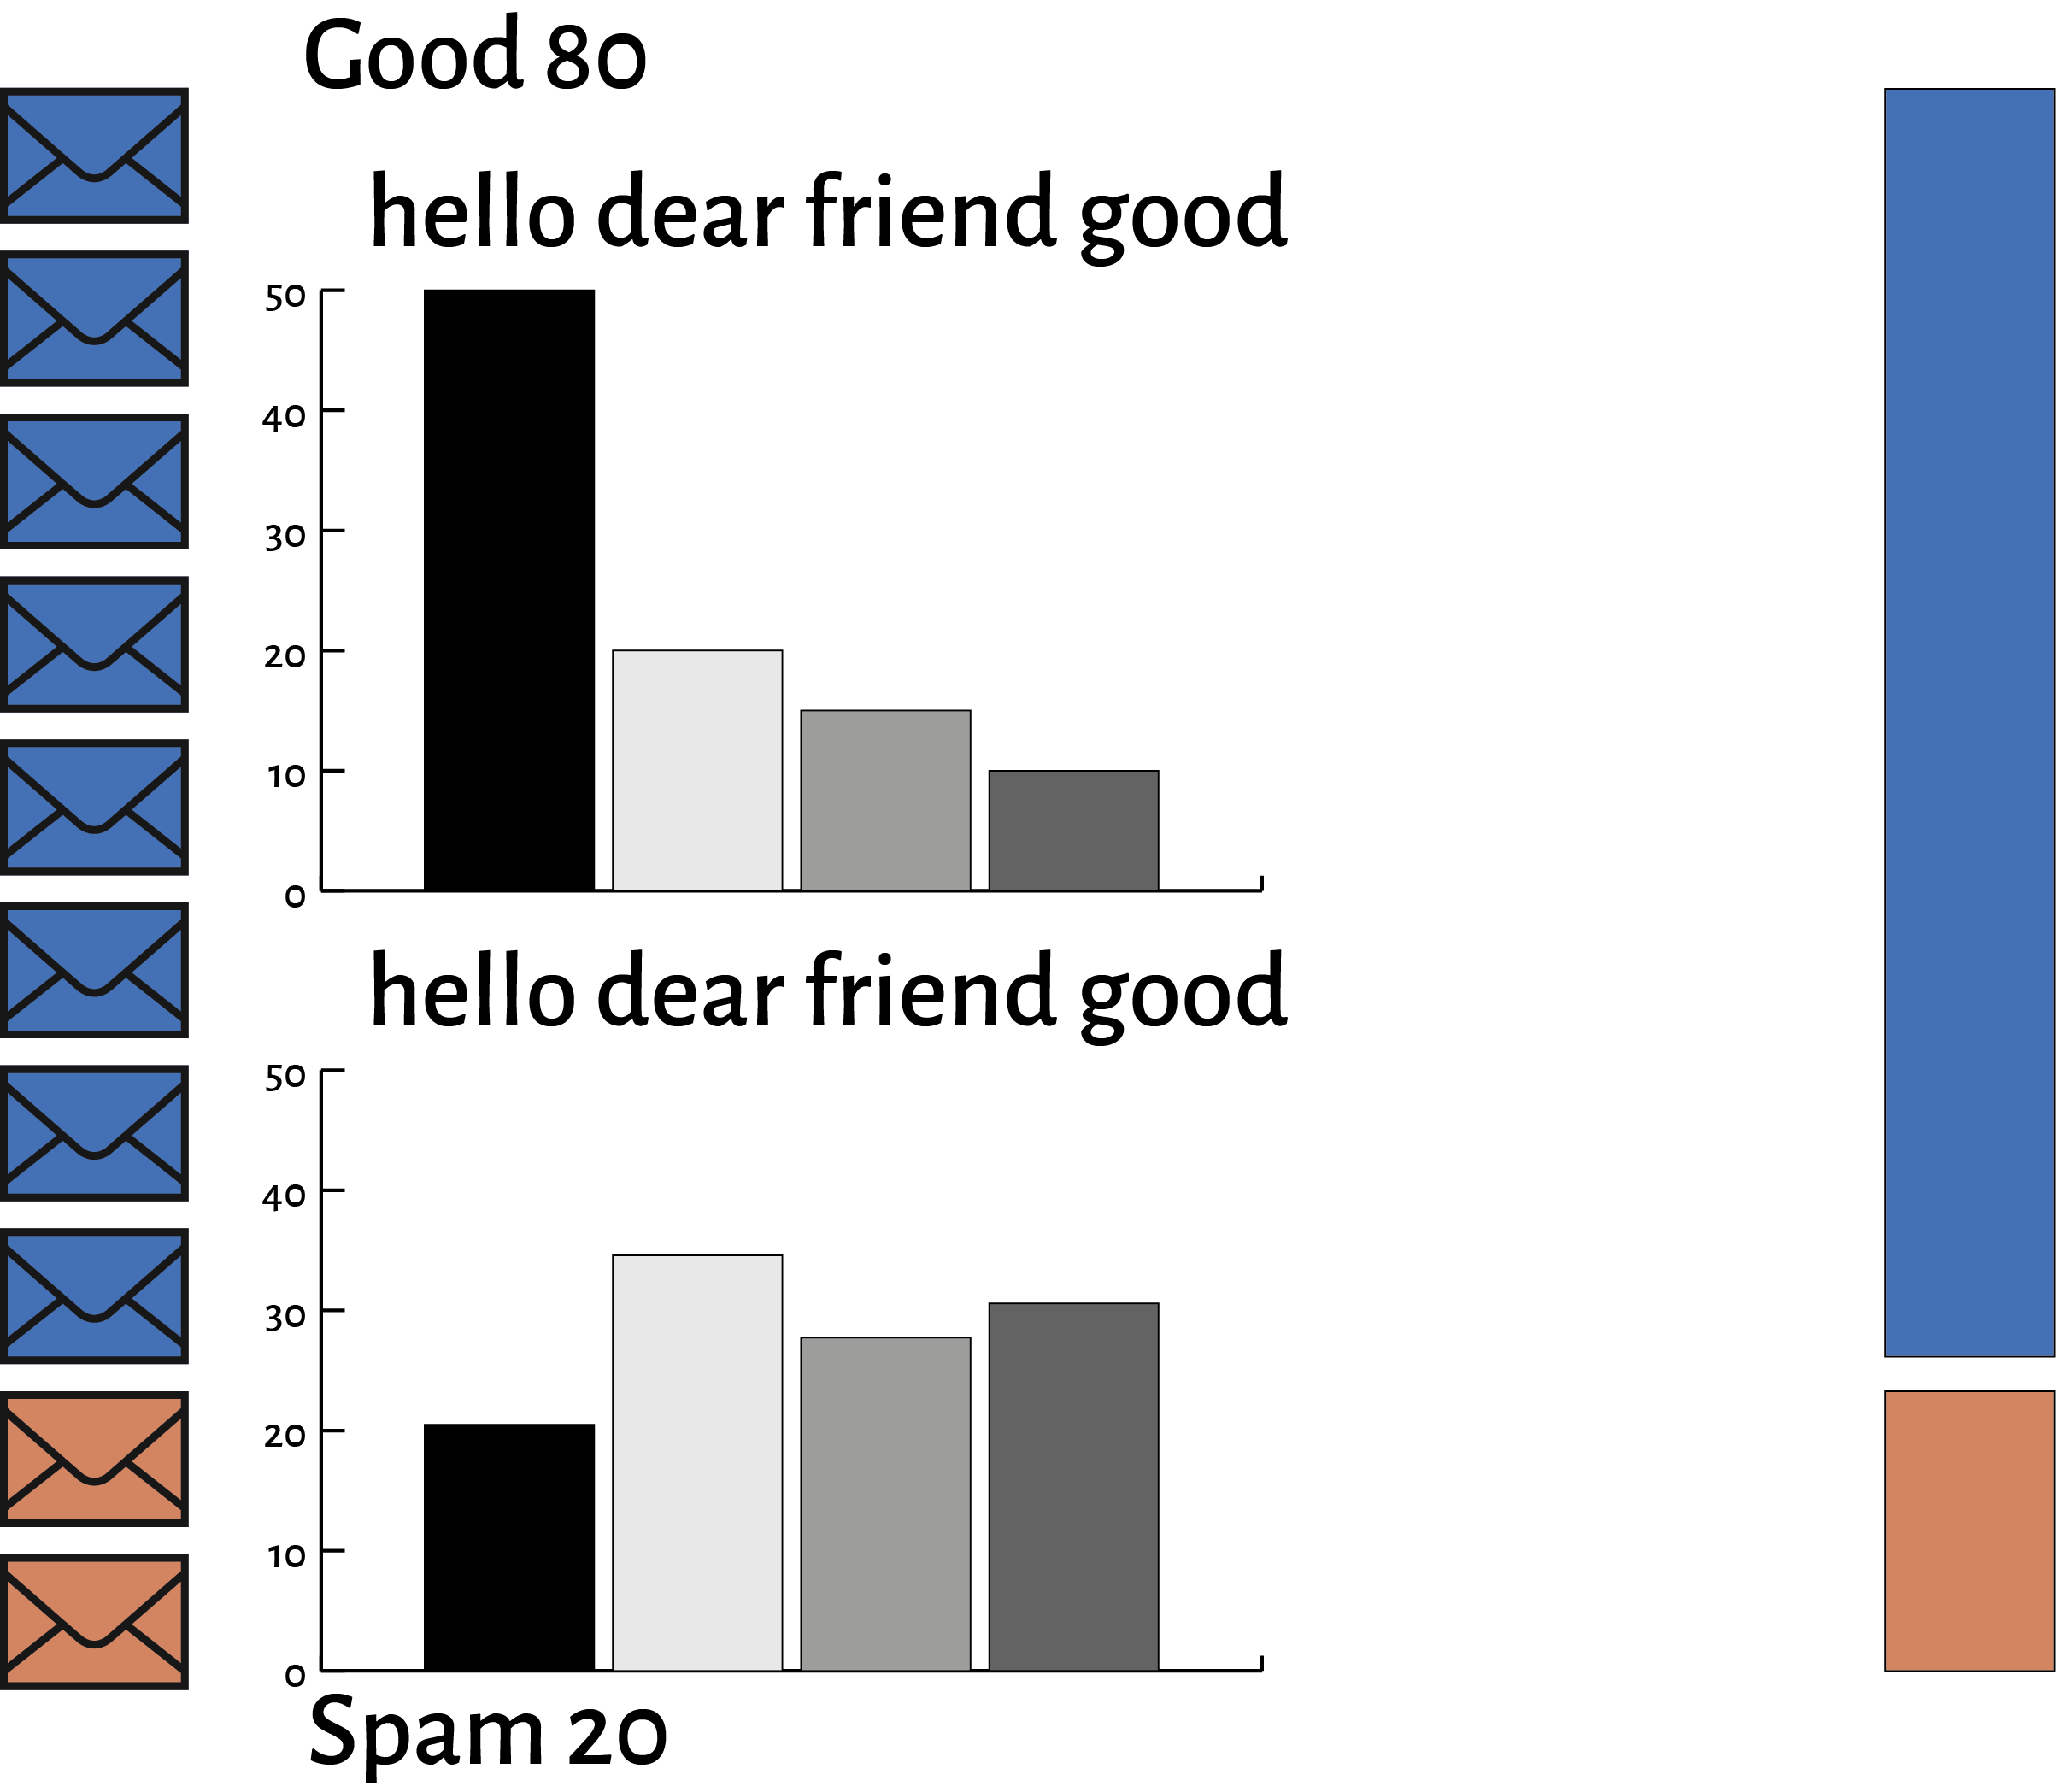
\includegraphics[width=0.8\textwidth,keepaspectratio]{images/spam02}
        \caption{}
        \label{fig:spam02}
    \end{figure}
\end{frame}

\begin{frame}[fragile]
    \frametitle{Python Example}
    \begin{lstlisting}[style=pythonStyle, caption=Naive Bayes Classification Example]
    from sklearn.feature_extraction.text import CountVectorizer
    from sklearn.naive_bayes import MultinomialNB
    from sklearn.pipeline import make_pipeline
    from sklearn.datasets import fetch_20newsgroups
    data = fetch_20newsgroups(subset='train')
    X, y = data.data, data.target
    model = make_pipeline(CountVectorizer(), MultinomialNB())
    model.fit(X, y)
    new_text = ["This is a new text sample."]
    prediction = model.predict(new_text)
    print(f'Predicted category: {data.target_names[prediction[0]]}')
    \end{lstlisting}
\end{frame}

\begin{frame}
    \frametitle{Advantages and Disadvantages}
    \begin{itemize}
        \item \textbf{Advantages:}
        \begin{itemize}
            \item Simple and fast.
            \item Performs well with large datasets.
            \item Works well even with a small amount of training data.
        \end{itemize}
        \item \textbf{Disadvantages:}
        \begin{itemize}
            \item Assumption of feature independence can be unrealistic.
            \item May not perform well with highly correlated features.
        \end{itemize}
    \end{itemize}
\end{frame}

\begin{frame}
    \frametitle{Naive Bayes conclusion}
    \begin{itemize}
        \item Naive Bayes is a powerful and straightforward classification algorithm.
        \item It is especially useful for text classification problems in NLP.
        \item Understanding its assumptions and limitations is crucial for effective use.
    \end{itemize}
\end{frame}

\section{TF-IDF}

\begin{frame}
    \frametitle{TF-IDF Introduction}
    \begin{itemize}
        \item TF-IDF stands for Term Frequency-Inverse Document Frequency.
        \item It is a numerical statistic used to reflect the importance of a word in a document relative to a collection of documents (corpus).
        \item Commonly used in text mining and information retrieval.
    \end{itemize}
\end{frame}

\begin{frame}
    \frametitle{Term Frequency (TF)}
    \begin{block}{Definition}
        Term Frequency measures how frequently a term occurs in a document.
        \[
        \text{TF}(t, d) = \frac{\text{Number of times term } t \text{ appears in document } d}{\text{Total number of terms in document } d}
        \]
    \end{block}
    \begin{itemize}
        \item The higher the term frequency, the more relevant the term is to the document.
        \item Normalization is used to adjust for document length.
    \end{itemize}
\end{frame}

\begin{frame}
    \frametitle{Inverse Document Frequency (IDF)}
    \begin{block}{Definition}
        Inverse Document Frequency measures how important a term is within the entire corpus.
        \[
        \text{IDF}(t, D) = \log \frac{\text{Total number of documents in corpus } D}{\text{Number of documents containing term } t}
        \]
    \end{block}
    \begin{itemize}
        \item Terms that appear in many documents are less informative.
        \item Helps to reduce the weight of common terms.
    \end{itemize}
\end{frame}

\begin{frame}
    \frametitle{TF-IDF Calculation}
    \begin{block}{Definition}
        TF-IDF combines TF and IDF to measure the importance of a term in a document relative to the corpus.
        \[
        \text{TF-IDF}(t, d, D) = \text{TF}(t, d) \times \text{IDF}(t, D)
        \]
    \end{block}
    \begin{itemize}
        \item A high TF-IDF score indicates a term is important to the document and not too common in the corpus.
        \item Useful for feature extraction in text classification and clustering.
    \end{itemize}
\end{frame}

\begin{frame}
    \frametitle{Example Calculation}
    \begin{itemize}
        \item Suppose we have a corpus with 100 documents.
        \item The term "data" appears 10 times in document \( d \) with 100 total words.
        \item "Data" appears in 30 documents in the corpus.
    \end{itemize}
    \begin{block}{Term Frequency (TF)}
        \[
        \text{TF}(\text{"data"}, d) = \frac{10}{100} = 0.1
        \]
        \end{block}
    \begin{block}{Inverse Document Frequency (IDF)}
        \[
        \text{IDF}(\text{"data"}, D) = \log \frac{100}{30} \approx 0.5229
        \]
        \end{block}
    \begin{block}{TF-IDF}
        \[
        \text{TF-IDF}(\text{"data"}, d, D) = 0.1 \times 0.5229 \approx 0.0529
        \]
        \end{block}
\end{frame}

% Co-Occurrence Counts Slide
\begin{frame}
\frametitle{Co-Occurrence Counts}
Co-occurrence counts are used to build a term-document matrix:
\begin{itemize}
    \item Term-Document matrix: Each document is a count vector.
    \item Each word is a count vector in the vocabulary.
\end{itemize}
\[
\begin{tabular}{|c|c|c|c|}
\hline
\textbf{Counts} & \textbf{D1} & \textbf{D2} & \textbf{D3} \\
\hline
I & 1 & 1 & 1 \\
like & 1 & 1 & 0 \\
NLP & 0 & 0 & 1 \\
deep & 1 & 0 & 0 \\
learning & 1 & 0 & 0 \\
news & 0 & 1 & 0 \\
cooking & 0 & 0 & 1 \\
. & 1 & 1 & 1 \\
\hline
\end{tabular}
\]
\end{frame}

% Similarity Measurement Slide
\begin{frame}
\frametitle{Similarity Measurement}
Given two word vectors \( \mathbf{v}_1 \) and \( \mathbf{v}_2 \), similarity can be measured using the dot product:
\[
\mathbf{v}_1 \cdot \mathbf{v}_2 = \sum_{i=1}^{n} v_{1i} v_{2i}
\]
\begin{itemize}
    \item Dot product is longer if the vector is longer.
    \item The length of a vector represents the word's frequency.
    \item Longer length means the word occurs more frequently.
\end{itemize}
\end{frame}

% Cosine Similarity Slide
\begin{frame}
\frametitle{Cosine Similarity}
Cosine similarity normalizes similarity by vector length. In practice, we often use:
\[
\text{Cosine Similarity}(\mathbf{v}_1, \mathbf{v}_2) = \frac{\mathbf{v}_1 \cdot \mathbf{v}_2}{\|\mathbf{v}_1\| \|\mathbf{v}_2\|}
\]
\begin{itemize}
    \item This is the cosine of the angle between the two vectors.
\end{itemize}
\end{frame}


\begin{frame}[fragile]
    \frametitle{Python Example}
    \begin{lstlisting}[style=pythonStyle, caption=TF-IDF Example in Python]
    from sklearn.feature_extraction.text import TfidfVectorizer

    # Sample documents
    documents = [
        "The quick brown fox jumps over the lazy dog.",
        "The dog barks at the mailman."
    ]

    # Create the TF-IDF model
    vectorizer = TfidfVectorizer()
    tfidf_matrix = vectorizer.fit_transform(documents)

    # Convert to array for easy viewing
    print(tfidf_matrix.toarray())

    # Display feature names (terms)
    print(vectorizer.get_feature_names_out())
    \end{lstlisting}
\end{frame}

\begin{frame}
    \frametitle{Applications}
    \begin{itemize}
        \item \textbf{Text Classification}: Assigning labels to documents based on their content.
        \item \textbf{Information Retrieval}: Ranking documents based on their relevance to a query.
        \item \textbf{Text Clustering}: Grouping similar documents based on their TF-IDF features.
    \end{itemize}
\end{frame}

\begin{frame}
\frametitle{TF-IDF Alternatives}
\centering
\begin{tabular}{|l|c|}
\hline
\textbf{Scheme} & \textbf{Formula} \\ \hline
\textbf{TF-IDF} & $w_{ij} = \log(f_{ij}) \times \log\left(\frac{N}{n_j}\right)$ \\ \hline
\textbf{TF-ICF} & $w_{ij} = \log(f_{ij}) \times \log\left(\frac{N}{f_j}\right)$ \\ \hline
\textbf{Okapi BM25} & $w_{ij} = IDF(t) \cdot \frac{\text{TF}(t,d) \cdot (k_1 + 1)}{\text{TF}(t,d) + k_1 \cdot \left(1 - b + b \cdot \frac{|d|}{\text{avgdl}}\right)}$ \\ \hline
\textbf{ATC} & $w_{ij} = \frac{\left(0.5 + 0.5 \cdot \frac{f_i}{\max_j}\right) \cdot \log\left(\frac{N}{n_j}\right)}{\sqrt{\sum_{i=1}^{N} \left(0.5 + 0.5 \cdot \frac{f_i}{\max_j}\right)^2 \cdot \log^2\left(\frac{N}{n_j}\right)}}$ \\ \hline
\vdots & \vdots \\ \hline
\end{tabular}
\end{frame}

% BM-25 Overview
\begin{frame}{BM-25 Overview}
    \begin{itemize}
        \item \textbf{BM-25:} An improvement over TF-IDF, it is a probabilistic-based ranking function.
        \item It considers term frequency saturation and document length normalization.
        \item Formula:
        \[
        \text{BM25}(t, d) = \sum_{t \in q} IDF(t) \cdot \frac{\text{TF}(t, d) \cdot (k_1 + 1)}{\text{TF}(t, d) + k_1 \cdot \left(1 - b + b \cdot \frac{|d|}{\text{avgdl}}\right)}
        \]
        \item Parameters:
        \begin{itemize}
            \item \(k_1\): Controls term frequency saturation.
            \item \(b\): Controls document length normalization.
        \end{itemize}
    \end{itemize}
\end{frame}

% Key Differences
\begin{frame}{TF-IDF vs BM-25}
    \begin{itemize}
        \item \textbf{TF-IDF:}
        \begin{itemize}
            \item Simpler and faster to compute.
            \item Treats term frequency linearly.
            \item No explicit document length normalization.
        \end{itemize}
        \item \textbf{BM-25:}
        \begin{itemize}
            \item More accurate in handling term frequency saturation.
            \item Adjusts for varying document lengths.
            \item Uses hyperparameters \(k_1\) and \(b\) for tuning.
        \end{itemize}
    \end{itemize}
\end{frame}

% Use Cases
\begin{frame}{Use Cases}
    \begin{itemize}
        \item \textbf{TF-IDF:}
        \begin{itemize}
            \item Useful for document classification.
            \item Text summarization.
            \item Simple search implementations.
        \end{itemize}
        \item \textbf{BM-25:}
        \begin{itemize}
            \item Widely used in search engines (e.g., Elasticsearch, Lucene).
            \item Effective for large-scale information retrieval.
            \item Suitable for modern search applications with longer documents.
        \end{itemize}
    \end{itemize}
\end{frame}

% Problems of Count-Based Representation Slide
\begin{frame}
\frametitle{Problems of Count-Based Representation}
Count-based distributional representation faces several issues:
\begin{itemize}
    \item Increases in size with vocabulary.
    \item Requires a lot of storage.
    \item Sparsity issues for less frequent words.
    \item Subsequent classification models will be less robust.
\end{itemize}
\end{frame}

% Conclusion
\begin{frame}{TF-IDF conclusion}
    \begin{itemize}
        \item TF-IDF and BM-25 are foundational in search algorithms.
        \item BM-25 is often preferred in real-world applications due to its flexibility and accuracy.
        \item Understanding both models is key to improving search engine performance.
    \end{itemize}
\end{frame}

\begin{frame}{PageRank introduction}
    \begin{itemize}
        \item \textbf{PageRank:} A link analysis algorithm used by search engines to rank web pages.
        \item Developed by Larry Page and Sergey Brin at Stanford University.
        \item Based on the idea that important pages are likely to be linked to by many other pages.
        \item Pages with higher PageRank scores are deemed more authoritative and relevant.
    \end{itemize}
\end{frame}

% PageRank Formula
\begin{frame}{PageRank Formula}
    \begin{itemize}
        \item \textbf{PageRank Formula:}
        \[
        PR(A) = \frac{1 - d}{N} + d \times \sum_{i=1}^{m} \frac{PR(P_i)}{L(P_i)}
        \]
        \item \textbf{Explanation:}
        \begin{itemize}
            \item \(PR(A)\): PageRank of page \(A\).
            \item \(d\): Damping factor (usually set to 0.85).
            \item \(N\): Total number of pages.
            \item \(m\): Number of incoming links to page \(A\).
            \item \(P_i\): A page linking to page \(A\).
            \item \(L(P_i)\): Number of outgoing links from page \(P_i\).
        \end{itemize}
        \item PageRank iteratively computes the ranking of pages based on the links between them.
    \end{itemize}
\end{frame}

\begin{frame}{PageRank conclusion}
    \begin{itemize}
        \item \textbf{Why PageRank is Important:}
        \begin{itemize}
            \item One of the earliest algorithms that considered the structure of the web as a graph.
            \item Helped Google become one of the most successful search engines.
            \item Led to advancements in link analysis and contributed to modern ranking algorithms.
        \end{itemize}
        \item \textbf{Limitations:}
        \begin{itemize}
            \item Can be manipulated by link farming (creating lots of backlinks artificially).
            \item Does not consider content relevance, focusing mainly on the link structure.
        \end{itemize}
    \end{itemize}
\end{frame}

% Introduction Slide
\section{N-gram models}

\begin{frame}{Language Models (LMs)}
    \begin{itemize}
        \item Language models can be divided into two types:
        \begin{itemize}
            \item \textbf{Count-based Models (N-gram or Statistical)}
            \begin{itemize}
                \item Markov assumption of order n
                \item Approximation using n-gram probabilities
            \end{itemize}
            \item \textbf{Neural Language Models}
            \begin{itemize}
                \item Based on neural networks
            \end{itemize}
        \end{itemize}
    \end{itemize}
\end{frame}

\begin{frame}
\frametitle{N-gram models introduction}
N-gram language models are probabilistic models used in natural language processing (NLP) to predict the next word in a sequence. They are based on the Markov assumption, which simplifies the prediction by considering only the last \( n-1 \) words.
\end{frame}

% N-gram Definition Slide
\begin{frame}
\frametitle{What is an N-gram?}
An N-gram is a contiguous sequence of \( n \) items from a given text or speech corpus.
\begin{itemize}
    \item Unigram: Sequence of 1 word (e.g., "I").
    \item Bigram: Sequence of 2 words (e.g., "I am").
    \item Trigram: Sequence of 3 words (e.g., "I am learning").
    \item N-gram: Sequence of \( n \) words (e.g., "I am learning NLP").
\end{itemize}
\end{frame}

% N-gram Language Model Slide
\begin{frame}
\frametitle{N-gram Language Models}
N-gram language models estimate the probability of a word given the previous \( n-1 \) words:
\[
P(w_i | w_{i-(n-1)}, \dots, w_{i-1}) = \frac{\text{Count}(w_{i-(n-1)}, \dots, w_i)}{\text{Count}(w_{i-(n-1)}, \dots, w_{i-1})}
\]
\begin{itemize}
    \item The model simplifies the prediction by assuming that the next word depends only on the previous \( n-1 \) words.
    \item Common choices of \( n \): 1 (Unigram), 2 (Bigram), 3 (Trigram).
\end{itemize}
\end{frame}

\begin{frame}{Log probs}
    \begin{itemize}
        \item It is better to work with \textbf{logarithms of probabilities}:
        \begin{itemize}
            \item \textbf{Avoid overflow}: Logarithmic values prevent very small probabilities from becoming too close to zero, which could lead to underflow.
            \item \textbf{Addition is faster than multiplication}: Instead of multiplying probabilities, we can sum their logarithms, which is computationally cheaper.
        \end{itemize}
        \vspace{0.5cm}
        \item Example of converting a probability product to a log-sum:
        \[
        \text{Original: } p_1 \times p_2 \times p_3 \times p_4
        \]
        \[
        \text{Log-space: } \log(p_1) + \log(p_2) + \log(p_3) + \log(p_4)
        \]
    \end{itemize}
\end{frame}

\begin{frame}{How to Generate Text Using N-gram LMs?}
    \begin{itemize}
        \item N-gram models estimate probabilities based on word history.
        \item Key assumption: the probability of a word depends on a fixed number of previous words (history).
    \end{itemize}
\end{frame}

% Example of N-gram Model Slide
\begin{frame}
\frametitle{Example of a Trigram Model}
Given a sequence of words: "I like to learn NLP," a trigram language model predicts the probability of the next word based on the previous two words.
\begin{itemize}
    \item \( P(\text{NLP} | \text{to}, \text{learn}) = \frac{\text{Count}(\text{to learn NLP})}{\text{Count}(\text{to learn})} \)
\end{itemize}
\end{frame}

\begin{frame}
\frametitle{Example of a Trigram Model}
\begin{figure}
    \centering
    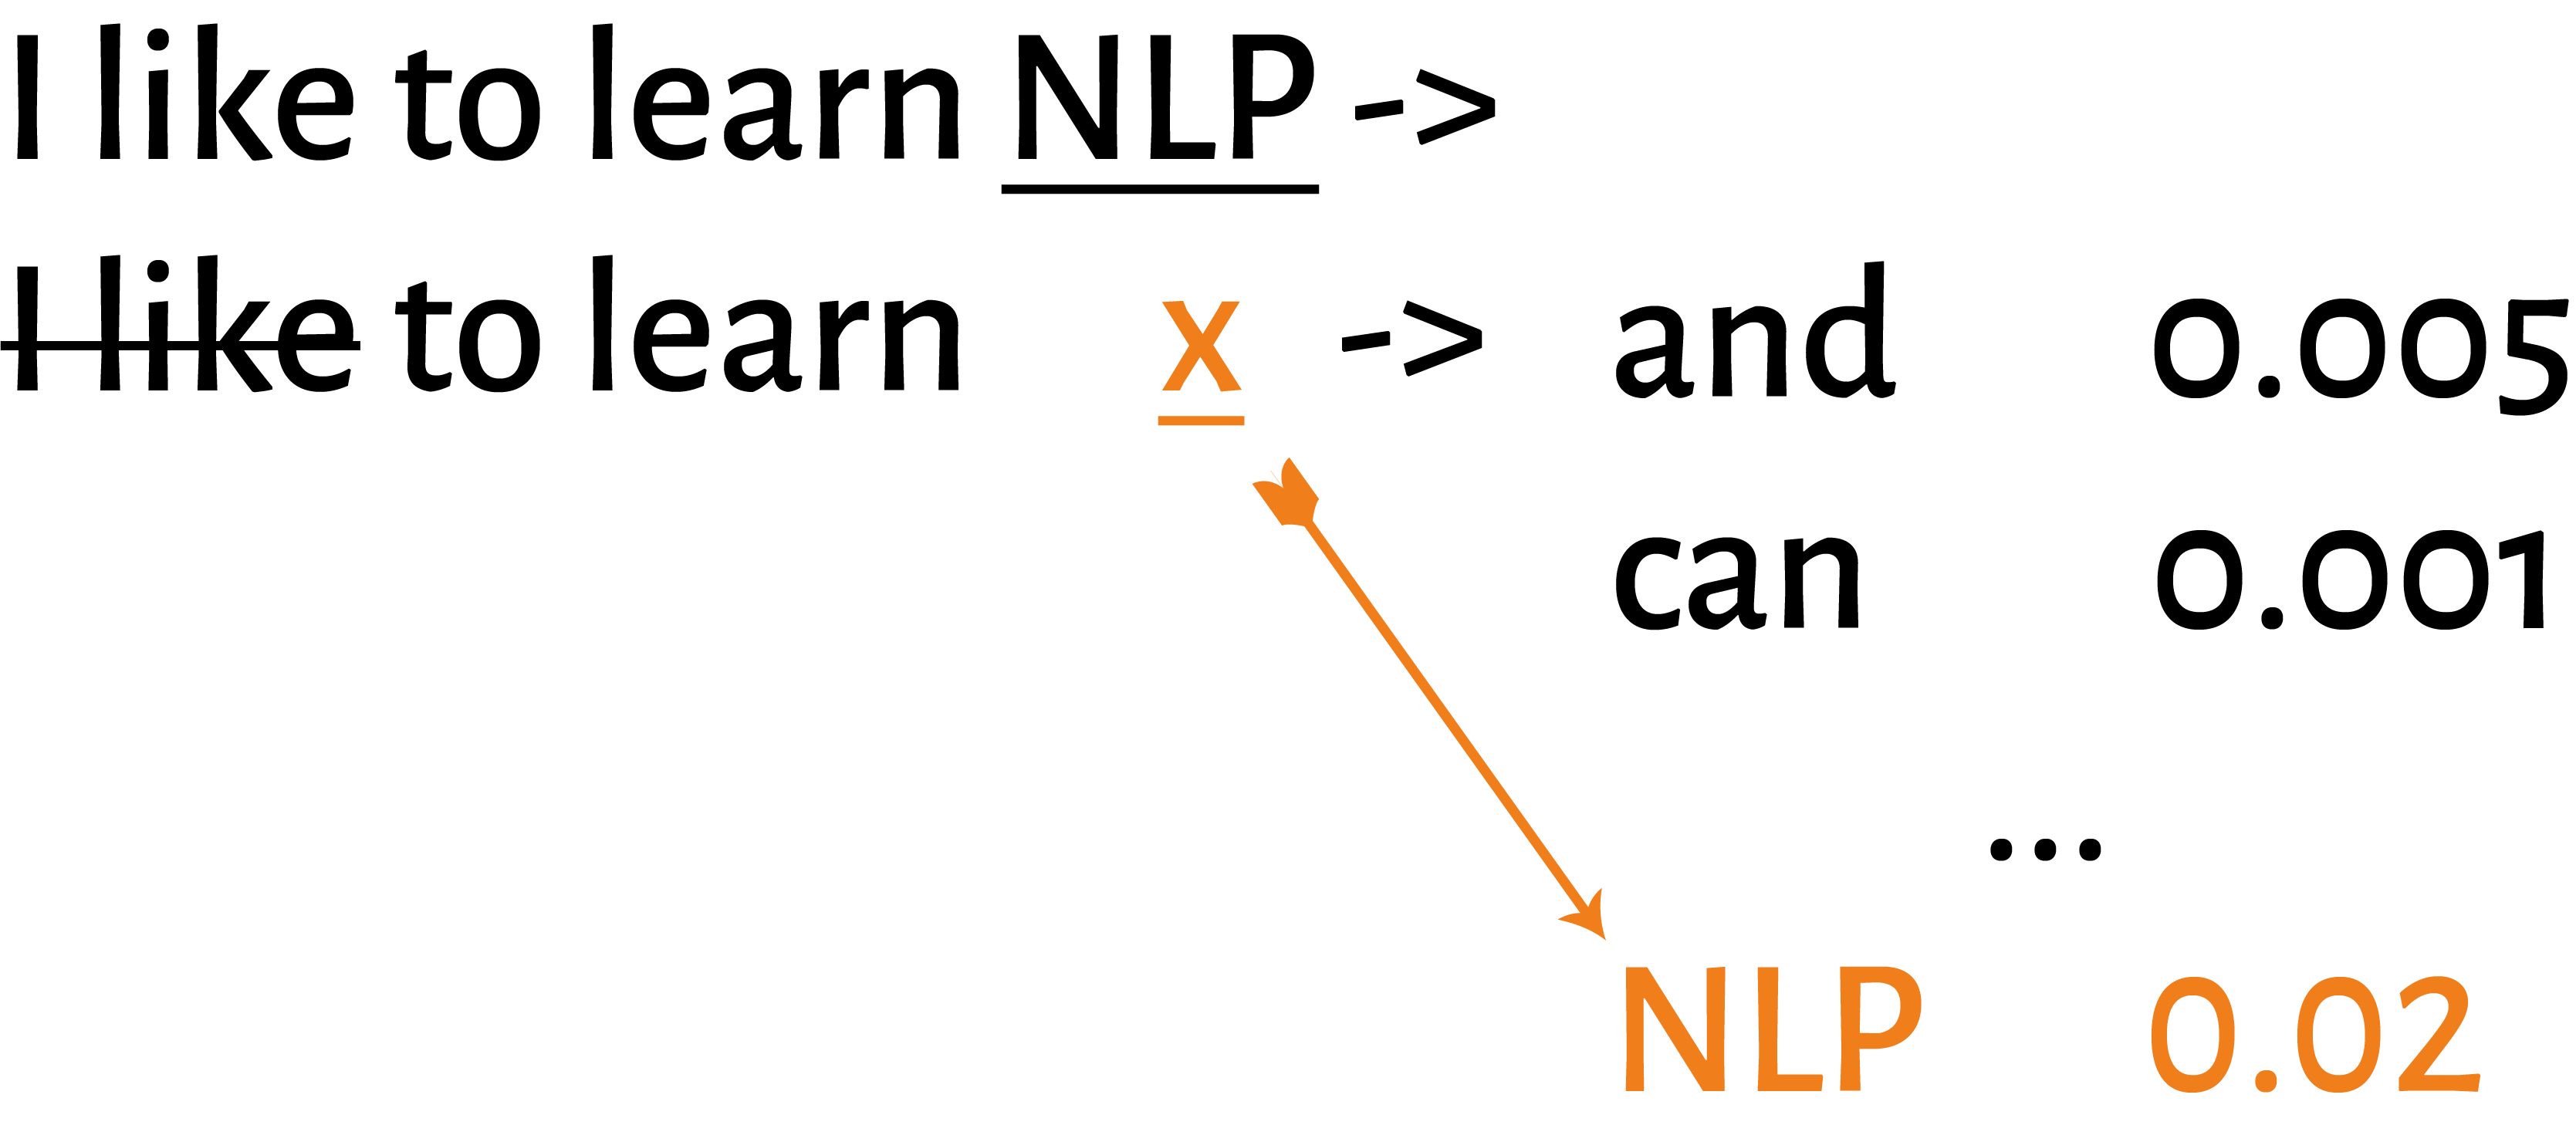
\includegraphics[width=0.5\textwidth,keepaspectratio]{images/n-gram_lm}
    \caption{N-gram LM}
    \label{fig:n-gram_lm}
\end{figure}

\end{frame}

% Smoothing in N-gram Models Slide
\begin{frame}
\frametitle{Smoothing in N-gram Models}
One challenge in n-gram models is handling unseen n-grams in the test data. Smoothing techniques address this issue by adjusting the probabilities:
\begin{itemize}
    \item Laplace Smoothing: Adds one to all counts to avoid zero probabilities.
    \item Add-k Smoothing: Generalization of Laplace, where \( k \) is added to each count.
    \item Backoff and Interpolation: Combine n-gram models of different orders to handle data sparsity.
\end{itemize}
\end{frame}

% Advantages and Disadvantages Slide
\begin{frame}
\frametitle{Advantages and Disadvantages}
\begin{itemize}
    \item Advantages:
    \begin{itemize}
        \item Simple to implement and understand.
        \item Effective for small to medium-sized datasets.
    \end{itemize}
    \item Disadvantages:
    \begin{itemize}
        \item Struggles with long-range dependencies.
        \item Data sparsity is a significant problem for larger \( n \).
        \item Exponential growth in the number of parameters with larger \( n \).
    \end{itemize}
\end{itemize}
\end{frame}

% Introduction Slide
\begin{frame}
\frametitle{Metrics overview}
Evaluating the quality of language models is crucial to understanding their performance in predicting sequences of words. Key measures for n-gram language models include:
\begin{itemize}
    \item Perplexity
    \item Cross-Entropy
    \item Precision, Recall, and F1 Score
\end{itemize}
These metrics help in comparing different models and selecting the best one for a given task.
\end{frame}

% Perplexity Slide
\begin{frame}
\frametitle{Perplexity}
Perplexity is a common evaluation metric for language models. It measures how well a language model predicts a test set.
\begin{itemize}
    \item Lower perplexity indicates a better model.
    \item Perplexity is calculated as:
    \[
    \text{Perplexity}(W) = 2^{-\frac{1}{N} \sum_{i=1}^{N} \log_2 P(w_i | w_{i-(n-1)}, \dots, w_{i-1})}
    \]
    \item Intuitively, perplexity can be thought of as the weighted average branching factor of the model.
\end{itemize}
\end{frame}

% Cross-Entropy Slide
\begin{frame}
\frametitle{Cross-Entropy}
Cross-entropy measures the average number of bits required to encode a word in the test set, given the probabilities assigned by the model.
\begin{itemize}
    \item Cross-entropy is closely related to perplexity:
    \[
    H(W) = -\frac{1}{N} \sum_{i=1}^{N} \log_2 P(w_i | w_{i-(n-1)}, \dots, w_{i-1})
    \]
    \item Lower cross-entropy indicates that the model is assigning higher probabilities to the correct words.
    \item Cross-entropy is used in various tasks, including language modeling, machine translation, and speech recognition.
\end{itemize}
\end{frame}

% Precision, Recall, F1 Score Slide
\begin{frame}
\frametitle{Precision, Recall, and F1 Score}
These metrics can also be used to evaluate n-gram language models, particularly in the context of predicting specific words or phrases.
\begin{itemize}
    \item Precision: Measures the proportion of correct positive predictions:
    \[
    \text{Precision} = \frac{\text{True Positives}}{\text{True Positives} + \text{False Positives}}
    \]
    \item Recall: Measures the proportion of actual positives that were predicted correctly:
    \[
    \text{Recall} = \frac{\text{True Positives}}{\text{True Positives} + \text{False Negatives}}
    \]
    \item F1 Score: Harmonic mean of precision and recall, providing a single score for model performance:
    \[
    \text{F1 Score} = 2 \times \frac{\text{Precision} \times \text{Recall}}{\text{Precision} + \text{Recall}}
    \]
\end{itemize}
\end{frame}

%% Coverage Slide
%\begin{frame}
%\frametitle{Coverage}
%Coverage measures how well the model can capture the full range of n-grams present in the test data.
%\begin{itemize}
%    \item A model with good coverage assigns non-zero probabilities to a large proportion of the test data n-grams.
%    \item Poor coverage can lead to high perplexity, as the model fails to predict many unseen n-grams.
%\end{itemize}
%\end{frame}

%% Overfitting Slide
%\begin{frame}
%\frametitle{Overfitting}
%Overfitting occurs when a model performs well on the training data but poorly on unseen data.
%\begin{itemize}
%    \item Common in n-gram models with a high value of \( n \), as the model captures noise in the training data.
%    \item Regularization and smoothing techniques, such as Laplace or Kneser-Ney smoothing, help mitigate overfitting.
%\end{itemize}
%\end{frame}

% Conclusion Slide
\begin{frame}
\frametitle{Conclusion}
N-gram language models are foundational in NLP and are still used in various applications. While they are limited by their inability to capture long-range dependencies and suffer from data sparsity, they provide a simple and effective approach for language modeling, especially in resource-constrained environments.
\end{frame}

% References Slide
\begin{frame}
\frametitle{References}
\begin{itemize}
    \item Jurafsky, D., & Martin, J. H. (2020). \textit{Speech and Language Processing}. Stanford.
    \item Manning, C. D., Raghavan, P., & Schütze, H. (2009). \textit{Introduction to Information Retrieval}. Cambridge University Press.
\end{itemize}
\end{frame}

\section{SMT}

% Slide 1: Introduction to SMT
\begin{frame}{Introduction to Statistical Machine Translation (SMT)}
    \begin{itemize}
        \item \textbf{Statistical Machine Translation (SMT)}:
        \begin{itemize}
            \item Translates text based on statistical models derived from bilingual text corpora.
            \item Key assumption: the best translation maximizes the probability of the target sentence given the source sentence.
        \end{itemize}
        \item \textbf{Key Components}:
        \begin{itemize}
            \item Language model (LM)
            \item Translation model (TM)
            \item Decoding algorithm
        \end{itemize}
    \end{itemize}
\end{frame}

% Slide 2: Noisy Channel Model
\begin{frame}{Noisy Channel Model}
    \begin{itemize}
        \item The core idea behind SMT is the \textbf{Noisy Channel Model}:
        \[
        \hat{e} = \arg\max_{e} P(e | f)
        \]
        \item By Bayes' Theorem:
        \[
        P(e | f) = \frac{P(f | e) \cdot P(e)}{P(f)}
        \]
        \item The denominator \(P(f)\) is independent of \(e\), so we focus on maximizing:
        \[
        \hat{e} = \arg\max_{e} P(f | e) \cdot P(e)
        \]
        \begin{itemize}
            \item \(P(f | e)\): Translation model (TM)
            \item \(P(e)\): Language model (LM)
        \end{itemize}
    \end{itemize}
\end{frame}

% Slide 3: Language Model (LM)
\begin{frame}{Language Model (LM)}
    \begin{itemize}
        \item \textbf{Language Model (LM)}:
        \begin{itemize}
            \item Models the probability of a sequence of words in the target language.
            \item Typically based on \textbf{n-grams}.
            \item Example: For a trigram model,
            \[
            P(e) = P(e_1) \cdot P(e_2 | e_1) \cdot P(e_3 | e_1, e_2) \cdot \dots
            \]
        \end{itemize}
        \item Helps ensure that the generated translation is fluent and grammatically correct.
    \end{itemize}
\end{frame}

% Slide 4: Translation Model (TM)
\begin{frame}{Translation Model (TM)}
    \begin{itemize}
        \item \textbf{Translation Model (TM)}:
        \begin{itemize}
            \item Models the probability of translating a source sentence into a target sentence.
            \item Typically based on word alignments and phrase-based models.
            \item Example:
            \[
            P(f | e) = \prod_{i} P(f_i | e_i)
            \]
        \end{itemize}
        \item Captures the lexical and syntactic relationships between source and target languages.
    \end{itemize}
\end{frame}

% Slide 5: Decoding Algorithm
\begin{frame}{Decoding Algorithm}
    \begin{itemize}
        \item The \textbf{Decoding Algorithm}:
        \begin{itemize}
            \item Finds the most probable target sentence given the source sentence.
            \item Typically uses beam search or dynamic programming techniques.
        \end{itemize}
        \item Balances between the translation model and language model to generate coherent translations.
    \end{itemize}
\end{frame}

% Slide 6: Training SMT Models
\begin{frame}{Training SMT Models}
    \begin{itemize}
        \item \textbf{Training SMT Models}:
        \begin{itemize}
            \item Requires large bilingual corpora to estimate the translation model parameters.
            \item Alignment of words or phrases between source and target languages is a crucial step.
        \end{itemize}
        \item \textbf{EM Algorithm (Expectation-Maximization)}:
        \begin{itemize}
            \item Commonly used to estimate the parameters of translation models.
        \end{itemize}
    \end{itemize}
\end{frame}

% Slide 7: Challenges in SMT
\begin{frame}{Challenges in SMT}
    \begin{itemize}
        \item \textbf{Data sparsity}: Insufficient data for rare words or phrases.
        \item \textbf{Model complexity}: Balancing between translation accuracy and computational efficiency.
        \item \textbf{Handling long-range dependencies}: Difficulty in capturing relationships between distant words in sentences.
        \item \textbf{Domain adaptation}: Translating text in different domains (e.g., legal, medical) requires specific data.
    \end{itemize}
\end{frame}

% Slide 7: Challenges in SMT
\begin{frame}{SMT outdates...}
    \begin{figure}
        \centering
        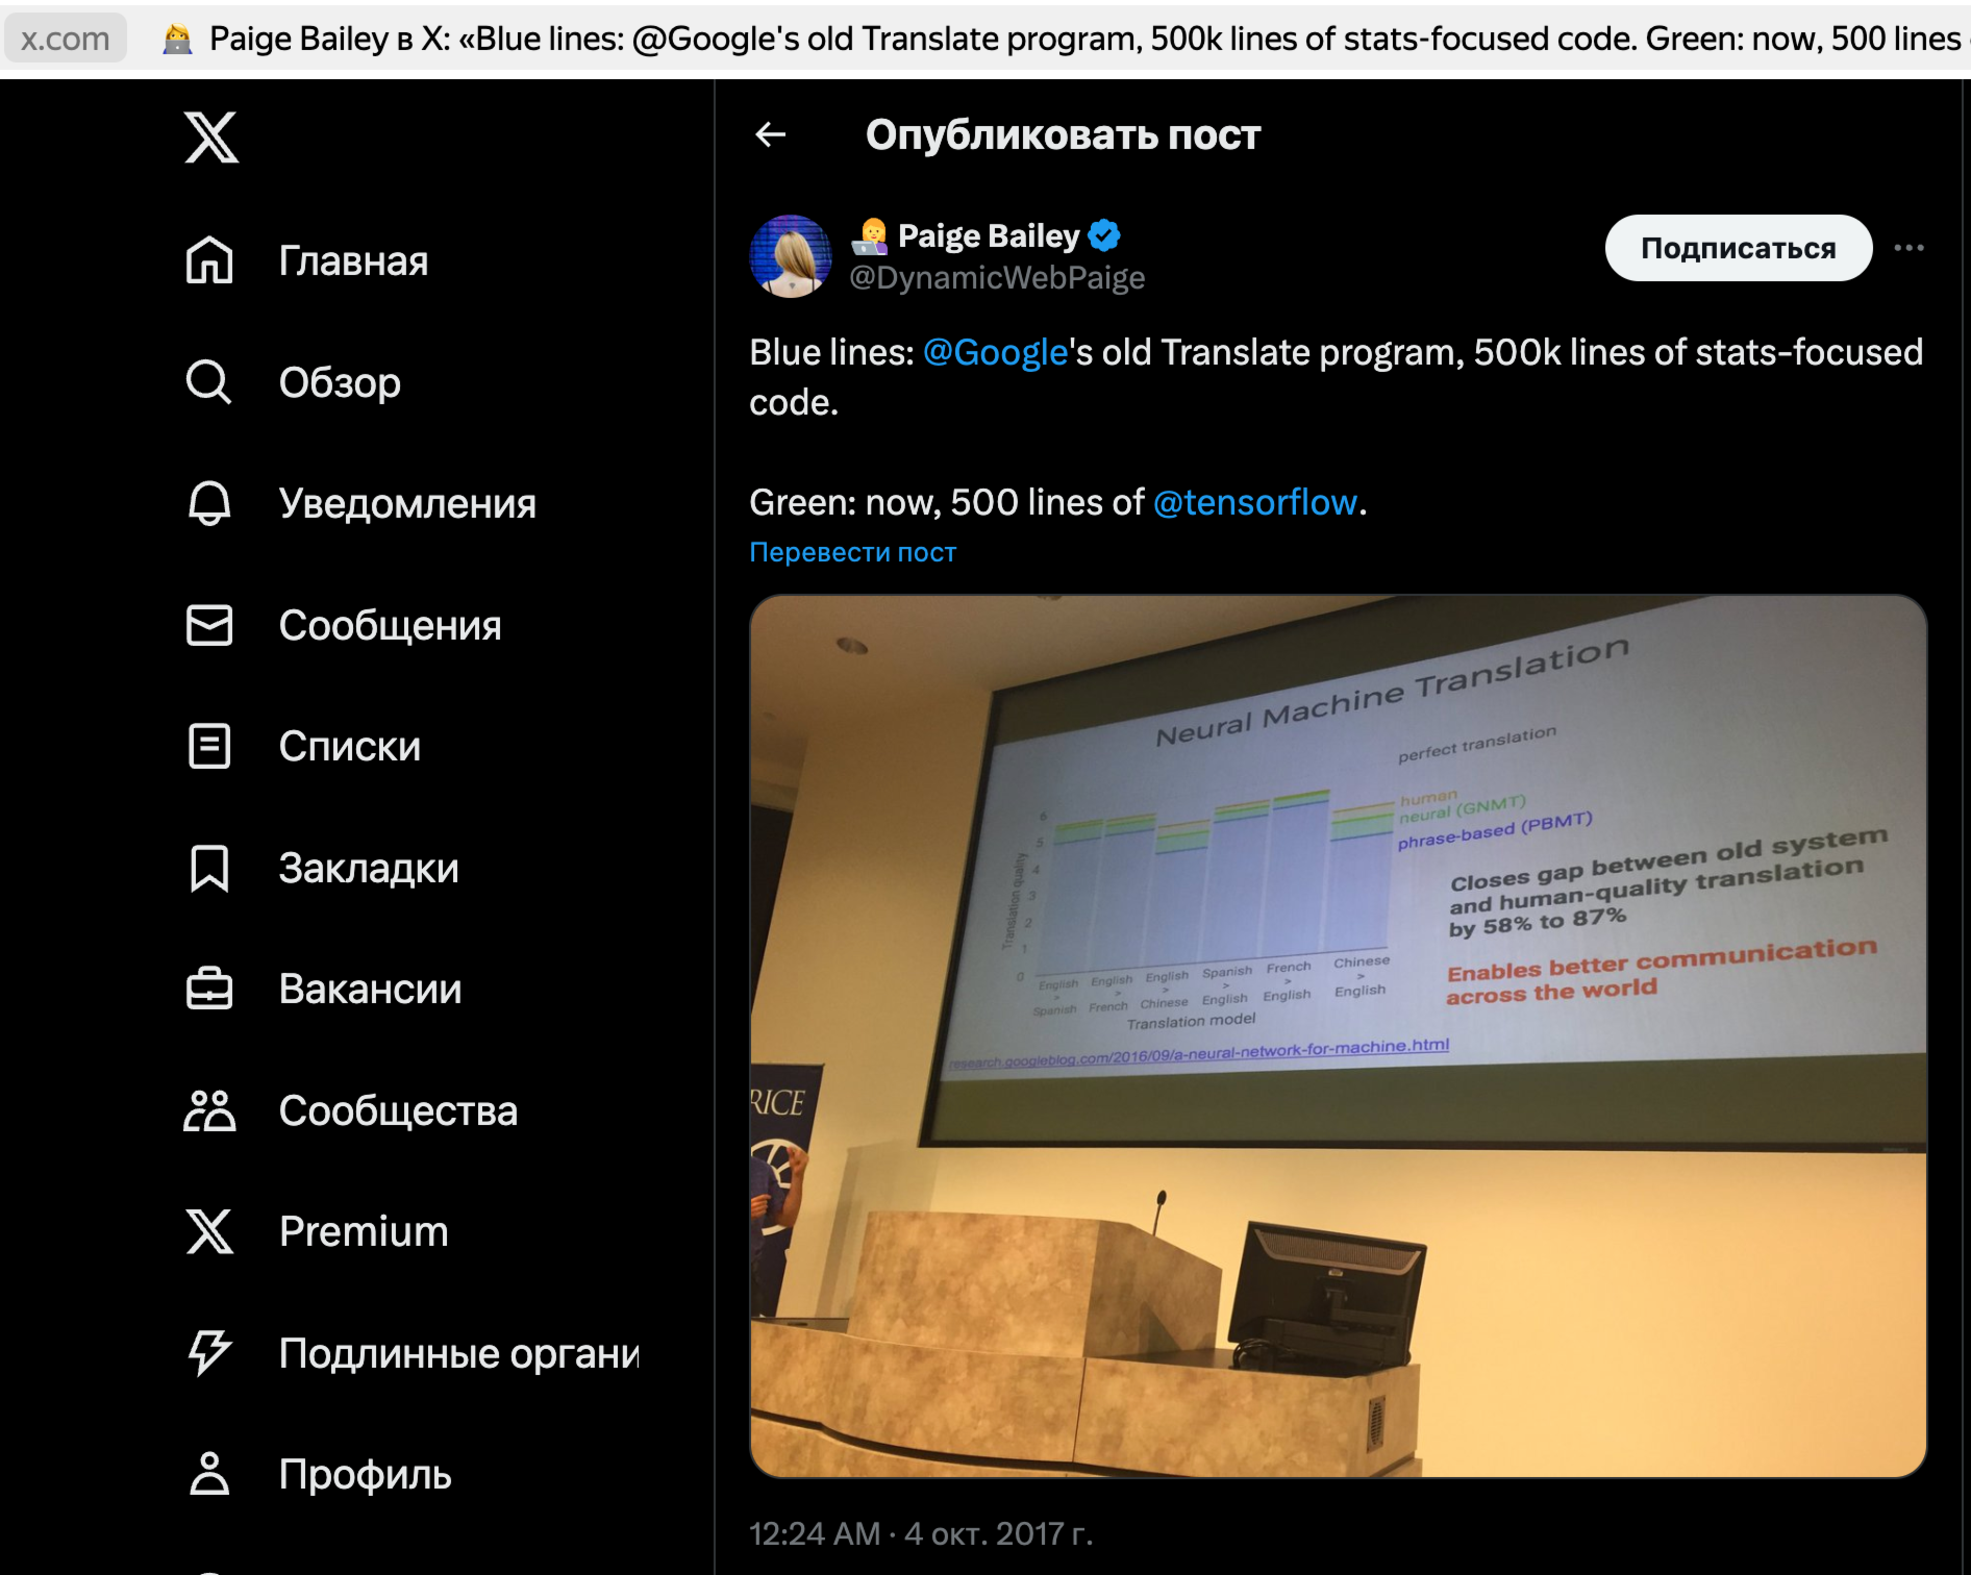
\includegraphics[width=0.9\textwidth,keepaspectratio]{images/500_lines}
        \caption{500 lines of RNN vs 500 000 of SMT}
        \label{fig:500_lines}
    \end{figure}

\end{frame}

% Slide 7: Challenges in SMT
\begin{frame}{Resources on SMT}
    \begin{itemize}
        \item \href{https://stepik.org/course/1233/syllabus}{курс Павла Браславского}
        \item \href{https://urss.ru/cgi-bin/db.pl?lang=Ru&blang=ru&page=Book&id=228448}{Прикладная и компьютерная лингвистика учебник}
    \end{itemize}
\end{frame}


\section{Seminar}
\begin{frame}
\frametitle{Seminar plan}
\begin{itemize}
    \item Regex
    \item Tokenization
    \item N-gram models
\end{itemize}
\end{frame}

\begin{frame}
\frametitle{Regex}
\begin{itemize}
    \item \href{https://habr.com/ru/articles/349860/}{Регулярные выражения в Python от простого к сложному}
    \item file 02\_seminar\_0\_regex.ipynb
\end{itemize}
\end{frame}

\begin{frame}
\frametitle{Tokenization}
\begin{itemize}
    \item file 02\_seminar\_02\_tokens\_normalization.ipynb
    \item \href{https://www.youtube.com/watch?v=zduSFxRajkE}{Let's build the GPT Tokenizer Andrei Karpatny}
\end{itemize}
\end{frame}

\begin{frame}
\frametitle{N-gram models}
\begin{itemize}
    \item 02\_seminar\_03\_ohe\_bow\_tf-idf\_search.ipynb
    \item \href{https://www.youtube.com/watch?v=PaCmpygFfXo}{The spelled-out intro to language modeling: building makemore Andrei Karpatny}
\end{itemize}
\end{frame}

\section{General Classification Framework in NLP}
\begin{frame}{General NLP Classification Framework}
    \begin{enumerate}
        \item Data Preprocessing
        \item Feature Extraction
        \item Model Selection
        \item Training
        \item Evaluation
    \end{enumerate}
\end{frame}

% Slide: Step 1 - Data Preprocessing
\begin{frame}{Step 1: Data Preprocessing}
    \begin{itemize}
        \item Tokenization: Breaking text into individual tokens (words, subwords).
        \item Stopword Removal: Removing common words like "the," "is."
        \item Stemming/Lemmatization: Reducing words to their base form.
        \item Lowercasing: Converting all words to lowercase.
    \end{itemize}
\end{frame}

% Slide: Step 2 - Feature Extraction
\begin{frame}{Step 2: Feature Extraction}
    \begin{itemize}
        \item Bag of Words (BoW): Counts word occurrences in a document.
        \item TF-IDF: Weights terms based on frequency across documents.
        \item Word Embeddings: Representing words in high-dimensional space (e.g., Word2Vec, GloVe).
        \item Sentence Embeddings: Representing entire sentences as vectors.
    \end{itemize}
\end{frame}

% Slide: Step 3 - Model Selection
\begin{frame}{Step 3: Model Selection}
    \begin{itemize}
        \item Traditional Models: Logistic Regression, SVM, Naive Bayes.
        \item Deep Learning Models: CNNs, RNNs, LSTMs, Transformers.
        \item Pretrained Models: BERT, GPT, RoBERTa.
    \end{itemize}
\end{frame}

% Slide: Step 4 - Model Training
\begin{frame}{Step 4: Model Training}
    \begin{itemize}
        \item Training Data: Labeled examples used to train the model.
        \item Optimization: Adjusting weights to minimize the loss (e.g., Adam, SGD).
        \item Hyperparameters: Tuning parameters such as learning rate, batch size.
    \end{itemize}
\end{frame}

% Slide: Step 5 - Model Evaluation
\begin{frame}{Step 5: Model Evaluation}
    \begin{itemize}
        \item Accuracy: Proportion of correct predictions.
        \item Precision & Recall: Metrics for evaluating class imbalance.
        \item F1 Score: Harmonic mean of precision and recall.
        \item Confusion Matrix: Breakdown of true positives, false positives, etc.
    \end{itemize}
\end{frame}

% Slide: Model - Neural Classifier
\begin{frame}{Neural Classifier}
    \begin{itemize}
        \item Define $h(x)$ as a feature extractor, where $x$ is the document from collection $X$.
        \item The goal is to predict the class $y$ as: \\
        $y = \arg\max P(y = k | h(x)) = \arg\max \logits_k$
        \item $\logits_k = w_a h(x)$, or in matrix form: $\logits = W h(x)$
        \item $y = \arg\max(\logits, \dim=-1)$
        \item Here, $h(x)$ is your favorite algorithm (including neural nets), serving as a feature extractor and generating a representation of text $x$.
    \end{itemize}
\end{frame}

% Slide: Cross-Entropy Loss
\begin{frame}{Cross-Entropy Loss}
    \begin{itemize}
        \item Neural classifiers are trained to predict probability distributions over classes.
        \item At each step, we maximize the probability a model assigns to the correct class.
        \item The standard loss function is the cross-entropy loss:
        \begin{align*}
        \text{Loss}(p^*, P) = - p^* \log(P)
        \end{align*}
        \item Here, $p^*$ is the target distribution (e.g., $(0,\dots, 0, 1, 0, \dots)$) and $P$ is the predicted distribution (e.g., $(P_1, P_2, ..., P_K)$).
    \end{itemize}
\end{frame}

% Slide: Conclusion
\begin{frame}{Classification Scheme}
    \begin{figure}
        \centering
        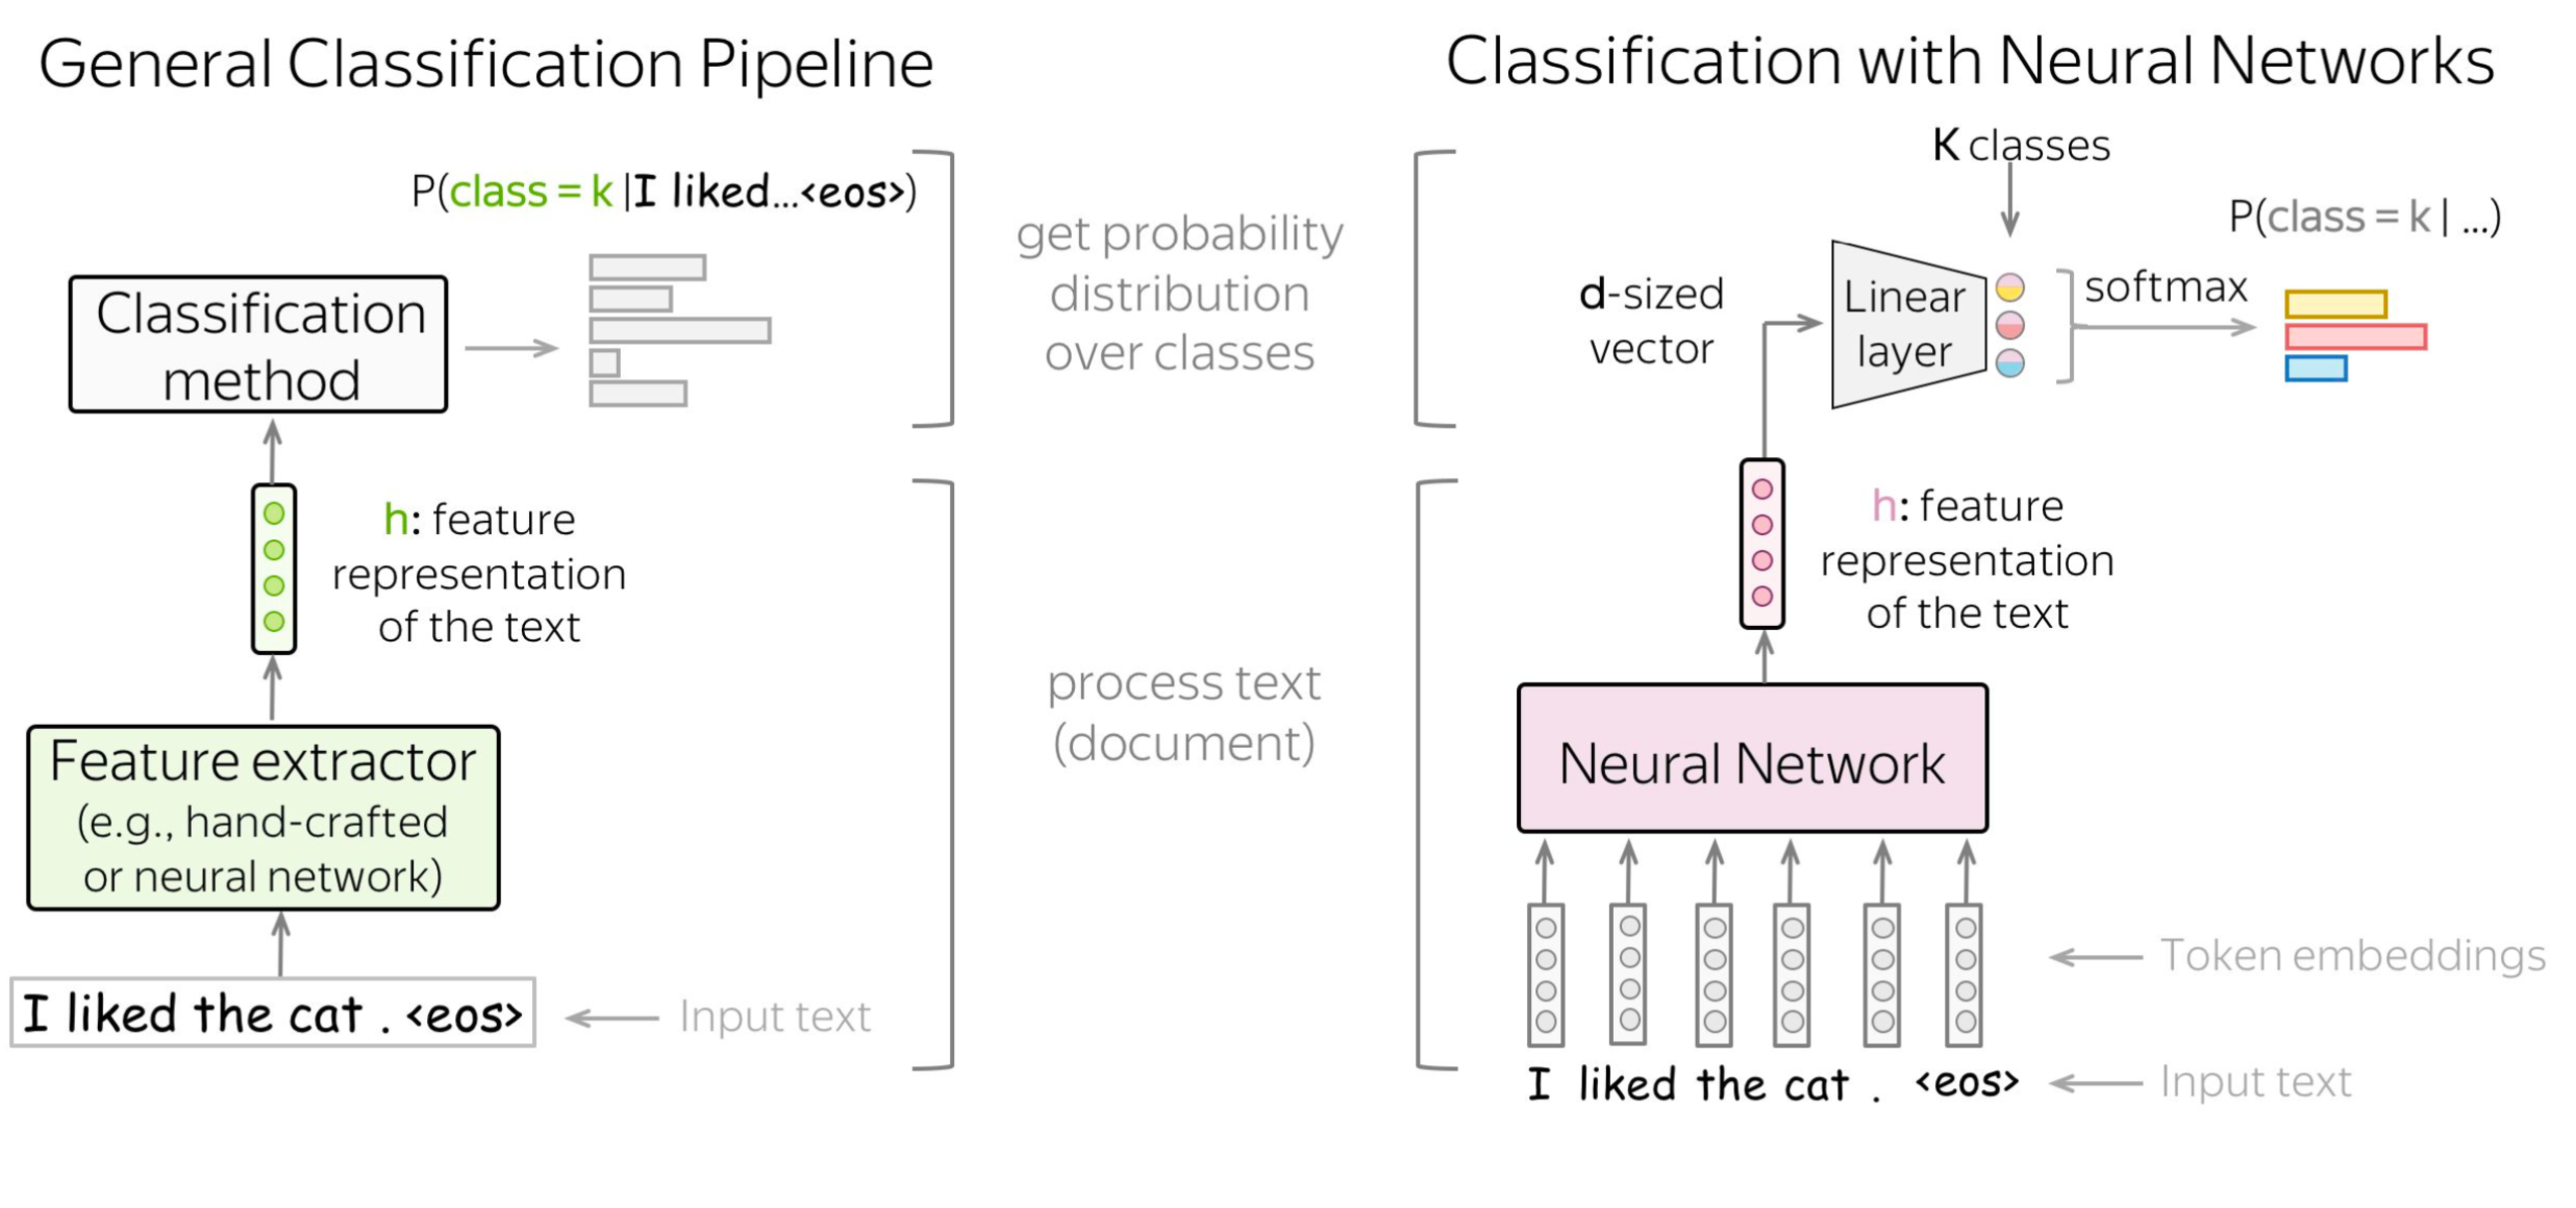
\includegraphics[width=1\textwidth,keepaspectratio]{images/classification_pipeline}
        \caption{Classification Scheme}
        \label{fig:classification_pipeline}
    \end{figure}
    
\end{frame}

\end{document}











